\documentclass{article}


% if you need to pass options to natbib, use, e.g.:
%     \PassOptionsToPackage{numbers, compress}{natbib}
% before loading neurips_2023


% ready for submission
% \usepackage[preprint]{neurips_2024}
\usepackage{iclr2025_conference,times}
\iclrfinalcopy

\theoremstyle{plain}
\newtheorem{theorem}{Theorem}
\newtheorem{lemma}{Lemma}[section]
\newtheorem{proposition}[lemma]{Proposition}
\newtheorem{corollary}[lemma]{Corollary}
\theoremstyle{definition}
\newtheorem{definition}[lemma]{Definition}
\newtheorem{assumption}[lemma]{Assumption}
\theoremstyle{remark}
\newtheorem{remark}[lemma]{Remark}


\newcommand{\diag}{\mathrm{diag}}
\newcommand{\norm}[1]{\left\|{#1}\right\|} %
\newcommand{\rank}{\mathrm{rank}}
\newcommand{\B}{\mathcal{B}}
\newcommand{\M}{\mathcal{M}}
\newcommand{\BS}{\B^*}
\newcommand{\BBS}{\B\B^*}
\newcommand{\BSB}{\B^*\B}
\newcommand{\MMS}{\M\M^*}
\newcommand{\MSM}{\M^*\M}
\newcommand{\BF}{\mathcal{B}\mathcal{F}}
\newcommand{\BD}{\mathcal{B}\mathcal{D}}
\newcommand{\DB}{\mathcal{D}\mathcal{B}}
\newcommand{\ind}[1]{^{(#1)}}

\newcommand{\vzero}{\mathbf{0}}
\newcommand{\vone}{\mathbf{1}}
\newcommand{\va}{\mathbf{a}}
\newcommand{\vb}{\mathbf{b}}
\newcommand{\vc}{\mathbf{c}}
\newcommand{\vd}{\mathbf{d}}
\newcommand{\ve}{\mathbf{e}}
\newcommand{\vf}{\mathbf{f}}
\newcommand{\vg}{\mathbf{g}}
\newcommand{\vh}{\mathbf{h}}
\newcommand{\vi}{\mathbf{i}}
\newcommand{\vj}{\mathbf{j}}
\newcommand{\vk}{\mathbf{k}}
\newcommand{\vl}{\mathbf{l}}
\newcommand{\vm}{\mathbf{m}}
\newcommand{\vn}{\mathbf{n}}
\newcommand{\vo}{\mathbf{o}}
\newcommand{\vp}{\mathbf{p}}
\newcommand{\vq}{\mathbf{q}}
\newcommand{\vr}{\mathbf{r}}
\newcommand{\vs}{\mathbf{s}}
\newcommand{\vt}{\mathbf{t}}
\newcommand{\vu}{\mathbf{u}}
\newcommand{\vv}{\mathbf{v}}
\newcommand{\vw}{\mathbf{w}}
\newcommand{\vx}{\mathbf{x}}
\newcommand{\vy}{\mathbf{y}}
\newcommand{\vz}{\mathbf{z}}
\newcommand{\vA}{\mathbf{A}}
\newcommand{\vB}{\mathbf{B}}
\newcommand{\vC}{\mathbf{C}}
\newcommand{\vD}{\mathbf{D}}
\newcommand{\vE}{\mathbf{E}}
\newcommand{\vF}{\mathbf{F}}
\newcommand{\vG}{\mathbf{G}}
\newcommand{\vH}{\mathbf{H}}
\newcommand{\vI}{\mathbf{I}}
\newcommand{\vJ}{\mathbf{J}}
\newcommand{\vK}{\mathbf{K}}
\newcommand{\vL}{\mathbf{L}}
\newcommand{\vM}{\mathbf{M}}
\newcommand{\vN}{\mathbf{N}}
\newcommand{\vO}{\mathbf{O}}
\newcommand{\vP}{\mathbf{P}}
\newcommand{\vQ}{\mathbf{Q}}
\newcommand{\vR}{\mathbf{R}}
\newcommand{\vS}{\mathbf{S}}
\newcommand{\vT}{\mathbf{T}}
\newcommand{\vU}{\mathbf{U}}
\newcommand{\vV}{\mathbf{V}}
\newcommand{\vW}{\mathbf{W}}
\newcommand{\vX}{\mathbf{X}}
\newcommand{\vY}{\mathbf{Y}}
\newcommand{\vZ}{\mathbf{Z}}

\newcommand{\cA}{\mathcal{A}}
\newcommand{\cB}{\mathcal{B}}
\newcommand{\cC}{\mathcal{C}}
\newcommand{\cD}{\mathcal{D}}
\newcommand{\cF}{\mathcal{F}}
\newcommand{\cG}{\mathcal{G}}
\newcommand{\cH}{\mathcal{H}}
\newcommand{\cI}{\mathcal{I}}
\newcommand{\cK}{\mathcal{K}}
\newcommand{\cL}{\mathcal{L}}
\newcommand{\cM}{\mathcal{M}}
\newcommand{\cN}{\mathcal{N}}
\newcommand{\cP}{\mathcal{P}}
\newcommand{\cS}{\mathcal{S}}
\newcommand{\cT}{\mathcal{T}}
\newcommand{\cX}{\mathcal{X}}

\newcommand{\R}{\mathbb{R}}
\newcommand{\F}{\mathbb{F}}

\newcommand{\Z}{\mathbb{Z}}
\newcommand{\ep}{\epsilon}
\newcommand{\g}{\gamma}
\newcommand{\Y}{\infty}
\newcommand{\f}[2]{\dfrac{#1}{#2}}
\newcommand{\ff}[2]{\tfrac{#1}{#2}}
\newcommand{\lm}[2]{\lim_{#1\rightarrow #2}}
\newcommand{\de}{\delta}
\newcommand{\T}{\theta}
\newcommand{\tm}{\times}
\newcommand{\su}[2]{\mathlarger{\sum\limits_{#1}^{#2}}}
\newcommand{\pd}[2]{\mathlarger{\prod\limits_{#1}^{#2}}}
\renewcommand{\sec}[1]{\section*{#1}}
\newcommand{\st}[1]{\subsection*{#1}}
\newcommand{\sst}[1]{\subsubsection*{#1}}
\renewcommand{\b}{\textbf}
\newcommand{\lessim}{\lesssim}
\newcommand{\E}{\mathbb{E}}
\newcommand{\p}{\partial}
\newcommand{\lt}{\left(}
\newcommand{\rt}{\right)}
\newcommand{\Lt}{\left[}
\newcommand{\Rt}{\right]}
\newcommand{\A}{\alpha}
\renewcommand{\b}{\beta}
\newcommand{\I}[2]{\mathlarger{\int_{#1}^{#2}}}
\newcommand{\G}{\nabla}
\newcommand{\Om}{\Omega}
\newcommand{\y}{\tau}
\newcommand{\K}{\mathcal{K}}
\newcommand{\C}{\mathbb{C}}
\newcommand{\om}{\omega}
\newcommand{\D}{\Delta}
\newcommand{\N}{\mathcal{N}}
\newcommand{\ra}{\rightarrow}
\newcommand{\Ra}{\Rightarrow}
\newcommand{\floor}[1]{\left\lfloor#1\right\rfloor}
\newcommand{\ceil}[1]{\left\lceil#1\right\rceil}
\newcommand{\ip}[1]{\left\langle#1\right\rangle}
\renewcommand{\mod}{\text{ mod }}
\newcommand{\sign}{\text{sign}}
\newcommand{\defeq}{:=}
\renewcommand{\a}{\bar{a}}
\newcommand{\MM}{\widetilde{\vM}}

\DeclareMathOperator*{\argmin}{argmin}


% to compile a preprint version, e.g., for submission to arXiv, add add the
% [preprint] option:
%     \usepackage[preprint]{neurips_2023}


% to compile a camera-ready version, add the [final] option, e.g.:
%     \usepackage[final]{neurips_2023}


% to avoid loading the natbib package, add option nonatbib:
%    \usepackage[nonatbib]{neurips_2023}

\usepackage[utf8]{inputenc} % allow utf-8 input
\usepackage[T1]{fontenc}    % use 8-bit T1 fonts
\usepackage{hyperref}       % hyperlinks
\usepackage{url}            % simple URL typesetting
\usepackage{booktabs}       % professional-quality tables
\usepackage{amsfonts}       % blackboard math symbols
\usepackage{nicefrac}       % compact symbols for 1/2, etc.
\usepackage{microtype}      % microtypography
\usepackage{xcolor}         % colors
\usepackage{graphicx}
\usepackage{multirow}
\usepackage{amsmath}        % aligned equations
\usepackage{bbm}
\usepackage{mathrsfs}
% \usepackage{emoji}
\usepackage{makecell}
\usepackage{subcaption} 
\usepackage{marvosym}
\usepackage{amsmath}
\usepackage{amssymb}

\newcommand{\tabincell}[2]{\begin{tabular}{@{}#1@{}}#2\end{tabular}} 

\usepackage{newfloat}
\usepackage{tcolorbox}
\usepackage{lipsum}
\usepackage{listings}
\usepackage{courier}
\usepackage{wrapfig}



\def\eg{\emph{e.g.}} \def\Eg{\emph{E.g.}}
\def\ie{\emph{i.e}} \def\Ie{\emph{I.e.}}
\def\cf{\emph{c.f.}} \def\Cf{\emph{C.f.}}
\def\etc{\emph{etc}} \def\vs{\emph{vs.}}
\def\wrt{w.r.t.} \def\dof{d.o.f.}
\def\etal{\emph{et al.}}


\title{UnrealZoo: Enriching Photo-realistic Virtual Worlds for Embodied AI}


\author{
Fangwei Zhong\textsuperscript{*$\sharp$$\dagger$}
Kui Wu\textsuperscript{*$\S$}
Churan Wang\textsuperscript{$\ddag$}
Hao Chen\textsuperscript{$\between$}
Hai Ci\textsuperscript{$\lozenge$}
Zhoujun Li\textsuperscript{$\S$}
Yizhou Wang\textsuperscript{$\ddag$}\\
\textsuperscript{$\sharp$} Beijing Normal University  
\textsuperscript{$\S$} Beihang University  
\textsuperscript{$\ddag$} Peking University 
\\
\textsuperscript{$\dagger$} BIGAI 
\textsuperscript{$\between$} City University of Macau  
\textsuperscript{$\lozenge$} National University of Singapore\\
\textsuperscript{*} indicates equal contribution, 
\Letter correspondence to: \texttt{fangweizhong@bnu.edu.cn} \\
}


\begin{document}


\maketitle

\vspace{-0.3cm}
\begin{abstract}

We introduce UnrealZoo~\footnote{Project page: \url{http://unrealzoo.site/}}, a rich collection of photo-realistic 3D virtual worlds built on Unreal Engine, designed to reflect the complexity and variability of the open worlds. Additionally, we offer a variety of playable entities for embodied AI agents. Based on UnrealCV, we provide a suite of easy-to-use Python APIs and tools for various potential applications, such as data collection, environment augmentation, distributed training, and benchmarking.
We optimize the rendering and communication efficiency of UnrealCV to support advanced applications, such as multi-agent interaction.
Our experiments benchmark agents in various complex scenes, focusing on visual navigation and tracking, which are fundamental capabilities for embodied visual intelligence.
The results yield valuable insights into the advantages of diverse training environments for reinforcement learning (RL) agents and the challenges faced by current embodied vision agents, including those based on RL and large vision-language models (VLMs), in open worlds. These challenges involve latency in closed-loop control in dynamic scenes and reasoning about 3D spatial structures in unstructured terrain.
\vspace{-0.3cm}
\end{abstract} 

\begin{figure*}[h]
    \centering
    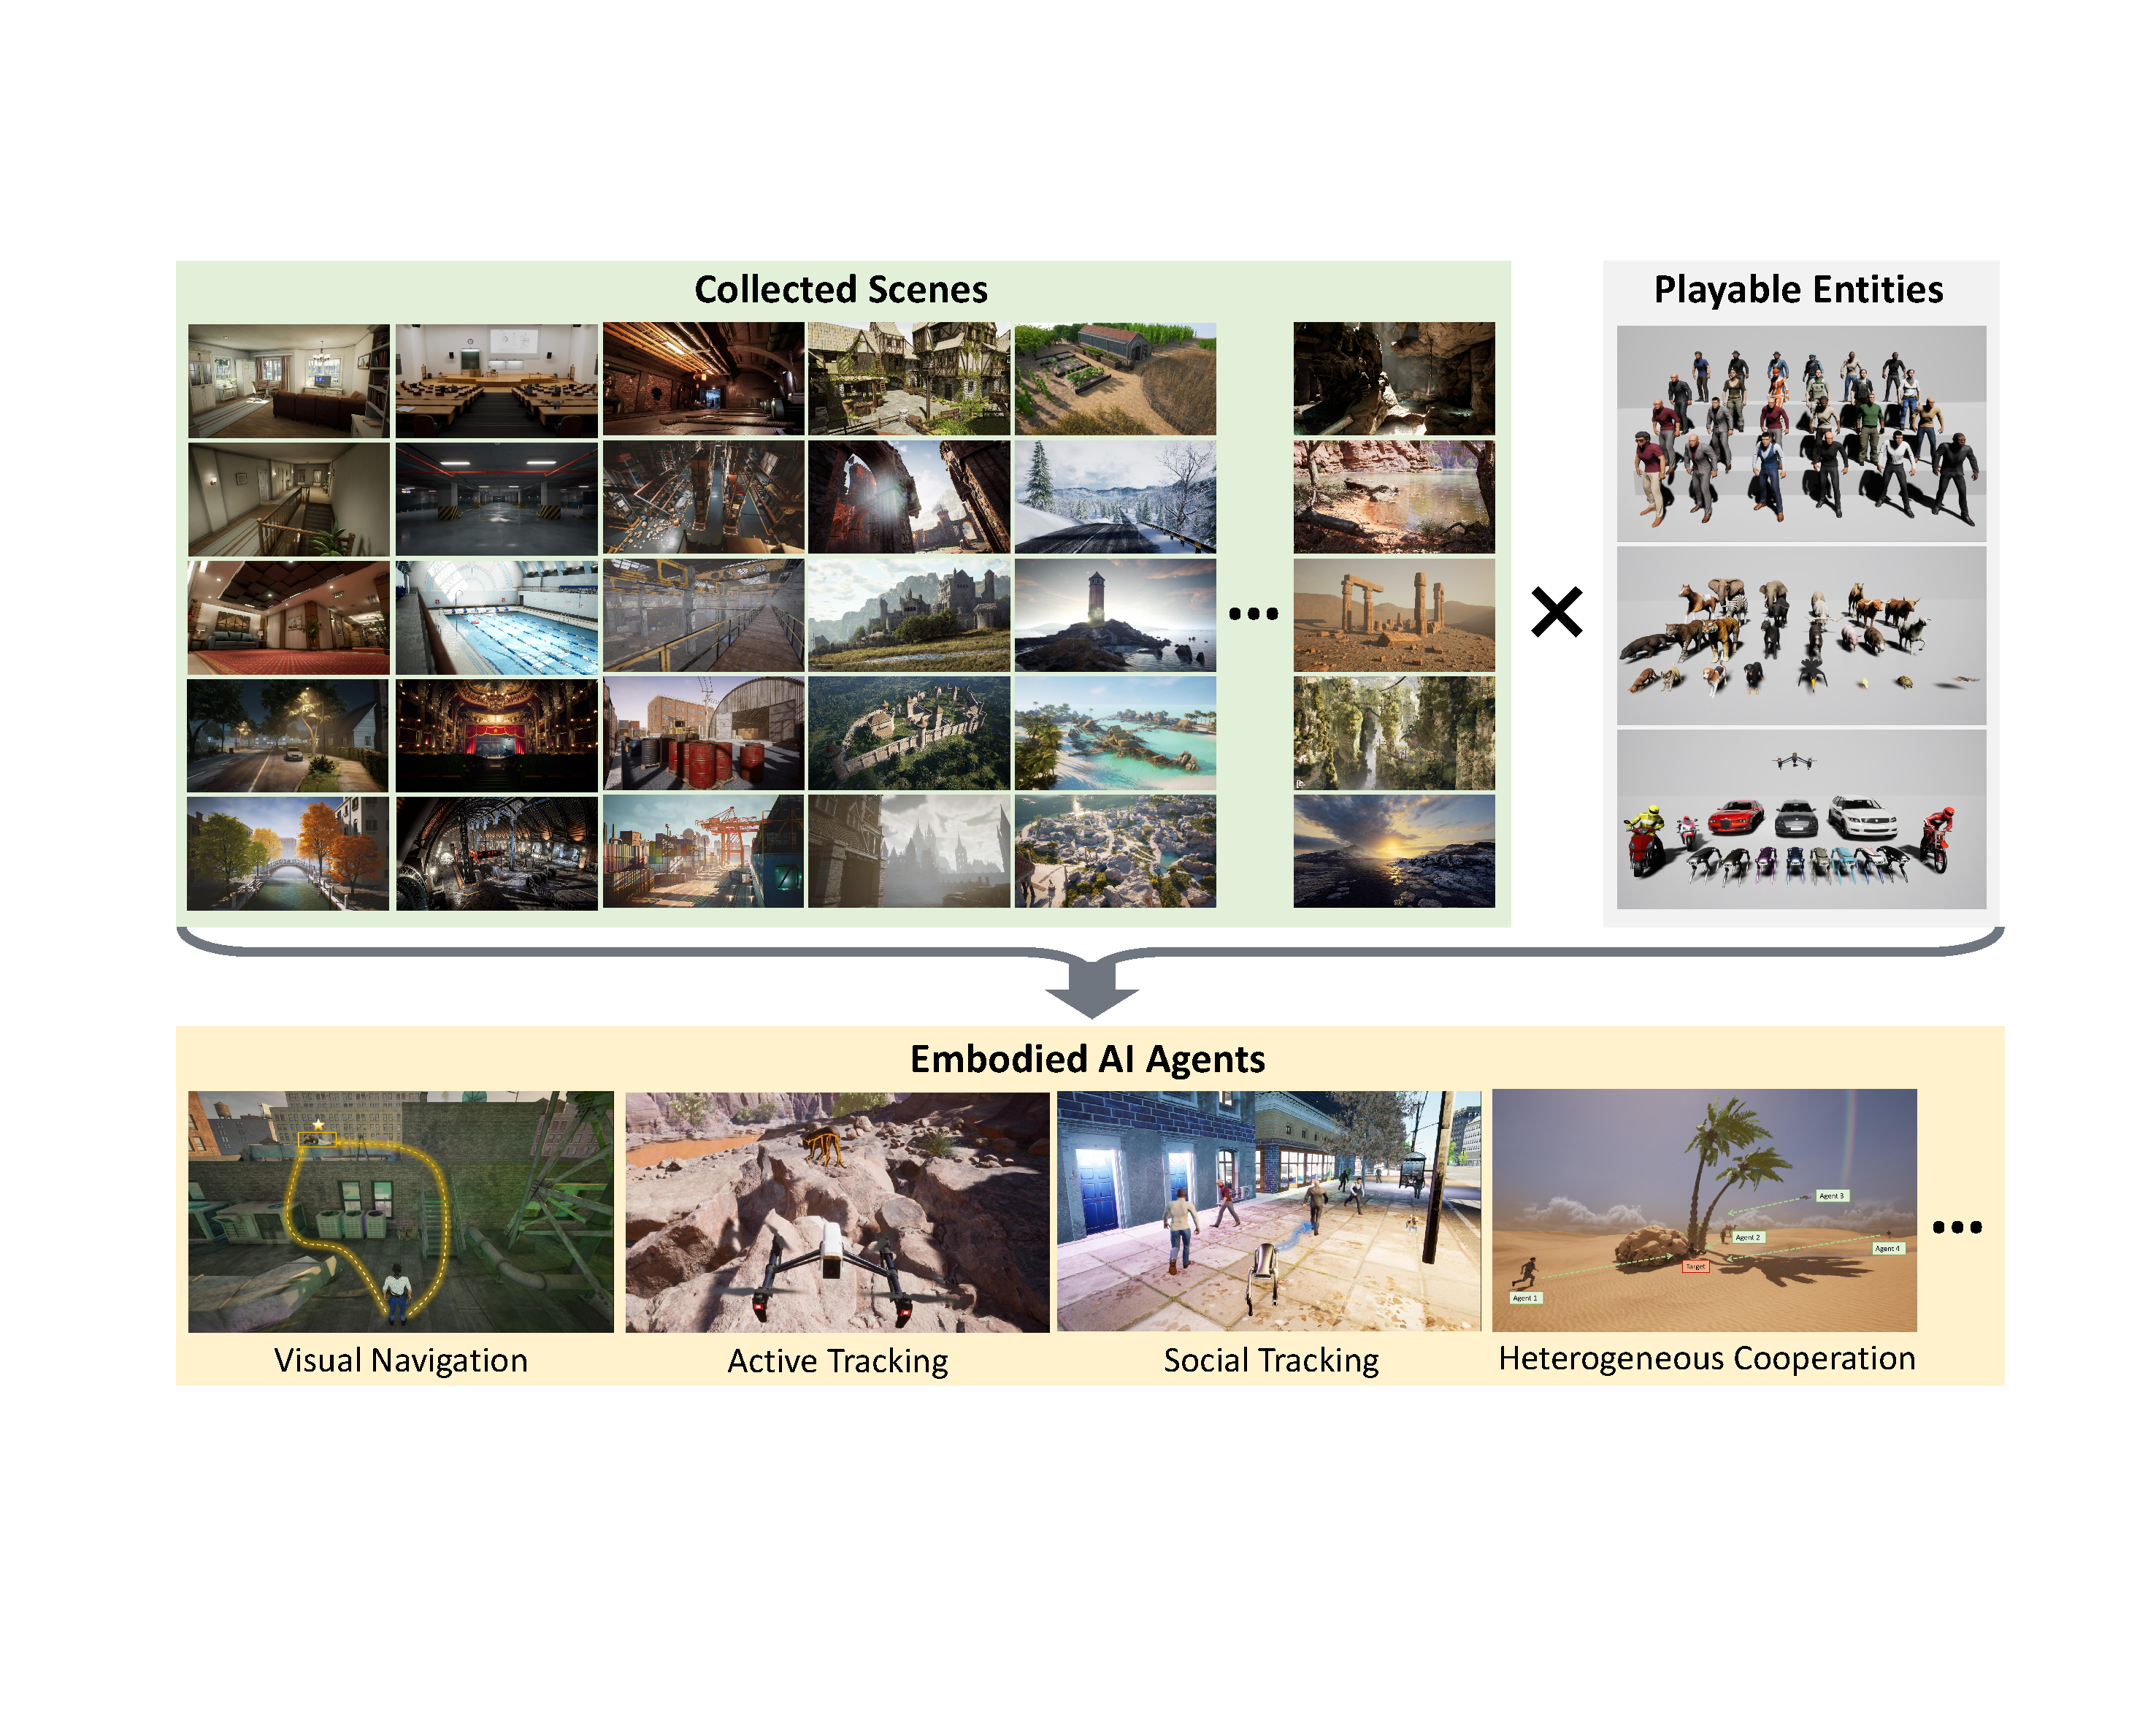
\includegraphics[width=0.99\textwidth]{image/overview2.pdf}
    \caption{
    UnrealZoo enriches photo-realistic virtual worlds by combining diverse scenes and playable entities. It enables training generalizable embodied AI agents for tasks such as navigation, active tracking, and social interactions. Additionally, UnrealZoo facilitates the benchmarking of agents in realistic virtual worlds, helping to identify challenges in open-world deployments.
    }
    \label{fig:overview}
\end{figure*}

\section{Introduction}


Currently, embodied artificial intelligence (Embodied AI) agents are often \textit{homebodies}, primarily confined to controlled indoor environments and rarely venturing outside to explore the diversity of the open world.  
While several simulators~\citep{kolve2017ai2, CARLA, puig2018virtualhome, li2023behavior,   puig2023habitat} have advanced the field, they often focus on specific scenarios, such as daily activities in homes or autonomous driving on urban roads.
This narrow focus hinders AI agents' adaptability and generalization in diverse open worlds, e.g., industrial areas, public spaces, and natural landscapes, required by a wide range of real-world applications.

To bridge this gap, there is an increasing demand for simulators that feature a diverse range of open worlds. 
\emph{First}, the diversity of the 3D scenes and bodies of agents is crucial to develop spatial intelligence~\citep{davison2018futuremapping}, enabling agents to actively perceive, reason, plan, and act when handling numerous tasks in complex 3D worlds with varying dynamics and styles.
\emph{Second}, the complexity of multi-agent interactions is essential for developing social intelligence~\citep{duenez2023social}, such as the theory of mind~\citep{jin-etal-2024-mmtom}, negotiation~\citep{guan2024richelieu}, cooperation~\citep{wang2022tomc}, and competition~\citep{zhong2021distractor}, encouraging agents to behave more like humans.
\emph{Third}, virtual worlds that mimic the challenges in open-world scenarios can evaluate agents efficiently and effectively, identifying limitations and preventing hardware losses from real-world deployment failures~\citep{kadian2020sim2real}.
\emph{Ultimately}, these features will inspire researchers to explore new challenges previously overlooked in other simulators~\citep{duan2022survey}, facilitating seamless integration into real-world applications.


In this work, we introduce UnrealZoo, a comprehensive collection of photo-realistic virtual worlds, based on Unreal Engine~\footnote{www.unrealengine.com} and UnrealCV~\citep{qiu2017unrealcv}. UnrealZoo features a diverse range of complex open worlds and playable entities to advance research in embodied AI and related domains. 
This high-quality set includes 100 realistic scenes at varying scales, such as houses, supermarkets, train stations, industrial factories, urban cities, villages, temples, and natural landscapes.
Each environment is expertly designed by artists to mimic realistic lighting, textures, and dynamics, closely resembling real-world experiences.
Our collection also includes diverse playable entities, including humans, animals, robots, drones, motorbikes, and cars. This diversity enables researchers to investigate the generalization of agents across different embodiments or build complex 3D social worlds with numerous heterogeneous agents.
To enhance usability, we further optimize UnrealCV and offer a suite of easy-to-use Python APIs and tools (UnrealCV+), including environment augmentation, demonstration collection, and distributed training/testing. These tools allow for customization and extension of the environments to meet various needs in future applications, ensuring UnrealZoo remains adaptable as the embodied AI agents evolve.

We conduct experiments to demonstrate the applicability of UnrealZoo for embodied AI. First, we benchmark frames per second (FPS) across various commands, highlighting the significant improvement in image rendering and multi-agent interactions with the UnrealCV+ API. We use embodied visual navigation~\citep{thor2017} and tracking~\citep{luo2018end, zhong2021distractor} as two example tasks to benchmark embodied vision agents in complex dynamic environments with moving objects and unstructured maps. We also introduce a set of simple yet effective baseline methods for developing embodied vision agents, including distributed online reinforcement learning algorithms~\citep{mnih2016asynchronous}, offline reinforcement learning algorithms~\citep{kumar2020conservative}, and a reasoning framework for large vision-language models (VLMs). Our evaluations across different settings emphasize the importance of diverse training environments for enhancing agent generalization and robustness, the necessity of low latency in closed-loop control to handle dynamic factors, and the potential of reinforcement learning for training agents to navigate complex scenes.

Our contributions can be summarized in the following:
1) We build UnrealZoo, a collection of 100 high-quality photo-realistic scenes and a set of playable entities with diverse features, covering the most challenging to embodied AI agents in open worlds.
2) We optimize the communication efficiency of UnrealCV APIs and provide easy-to-use Gym interfaces with a toolkit for diverse requirements.
3) We conduct experiments to demonstrate the usability of UnrealZoo, showing the importance of the diversity of the environments to the embodied agents, and analyzing the limitations of the current RL-based and VLM-based agents in the open worlds.



\section{Related Works}

\textbf{Realistic Simulators for Embodied AI.}
Realistic simulators are extensively utilized in embodied artificial intelligence due to their appealing benefits, including high-quality rendering, cost-effective ground truth generation, low-cost interaction, and environmental controllability. They are crucial for training and testing AI agents to handle increasingly complex tasks. Notable realistic 3D simulators have been created for specific applications, such as indoor navigation~\citep{kolve2017ai2, puig2018virtualhome, xia2018gibson, house3D}, robot manipulation~\citep{yu2020meta, ehsani2021manipulathor, chen2023bi}, and autonomous driving~\citep{virtual_kitti, airsim,  CARLA}.
Recent advances in computer graphics have spurred interest in developing general-purpose virtual worlds with photo-realistic rendering, allowing agents to collect high-fidelity data and learn skills applicable across various tasks and scenes. ThreeDWorlds (TDW)~\citep{gan2020threedworld} and LEGENT~\citep{cheng2024legent} are notable simulators that offer photo-realistic, multi-modal platforms, based on Unity, for interactive physical simulation. However, their built-in scenes and playable entities are somewhat limited. Additionally, the performance of the simulator decreases significantly in large outdoor environments, a typical weakness of Unity. V-IRL~\citep{yang2024v} is a recent approach that leverages Google Maps' API to simulate agents with real-world street view images, significantly reducing the gap between virtual and real-world settings. However, since V-IRL is inherently composed of static images, it lacks the capability to simulate the dynamics of the physical worlds for agent-object interactions.
Recently, the community has also begun to explore dynamic environments with social interactions and unexpected events. However, existing solutions like Habitat 3.0~\citep{puig2023habitat} focus on a limited number of agent interactions in indoor scenes, while HAZARD~\citep{zhou2024hazard} addresses only single-agent simulations in dynamic scenarios like fires, floods, and winds. In contrast, UnrealZoo offers a comprehensive collection of scenes that feature various scenes at different scales, situations, eras, and cultural backgrounds with diverse playable entities for embodied AI. With advancements in Unreal Engine and optimized UnrealCV, our environment achieves real-time performance in large-scale scenes with multiple agents (around 10) and photo-realistic rendering.
A comprehensive comparison across the related photo-realistic simulators is shown in Table~\ref{tab:env_comparision}.




\begin{table}[t]
\centering
    \caption{The comparison with related photo-realistic virtual worlds for embodied AI. \textbf{Unstr. Terr.} indicates the presence of unstructured terrain. \textbf{Nav. Sys.} specifies whether the agent in the environment includes an autonomous navigation system. In Appendix~\ref{app:env}, we compare the visual realism across different engines in Figure~\ref{fig: visual_realism} and list the descriptions of the symbols in Table~\ref{tab:symbol}.}
\label{tab:env_comparision}
\begin{tabular}{c}
\begin{minipage}{1\textwidth}
\includegraphics[width=\linewidth]{image/Compare_sim.pdf}
\end{minipage} 
\end{tabular}
\vspace{-0.5cm}
\end{table}


\renewcommand{\arraystretch}{1.1}

\textbf{Embodied Vision Agents.}
Embodied vision agents, which perceive and interact with their environments through vision, are a key focus in artificial intelligence research. These agents perform tasks like navigation~\citep{thor2017, gupta2017cognitive, yokoyama2024vlfm, long2024instructnav}, active object tracking~\citep{luo2018end, zhong2018advat, zhong2021distractor, zhong2023rspt, zhong2024empowering}, and other interactive tasks~\citep{chaplot2020learning, weihs2021visual, ci2023proactive, wang2023rearrange}, mimicking human behavior. Their development involves various methods, including state representation learning~\citep{yadav2023offline, yuan2022pre, gadre2022continuous, yang2023track}, reinforcement learning (RL)~\citep{schulman2017proximal, xu2023drm, ma2023revisiting}, and large vision-language models (VLMs)~\citep{zhang2024navid, zhou2024navgpt}.
Despite significant progress, challenges remain. RL methods often require extensive trial-and-error interactions and computational resources for training, and they usually struggle to generalize to new environments. Conversely, VLM-based methods excel at interpreting language instructions and images but may lack the fine-grained control and adaptability necessary for real-time interactions. The computational demands and time needed for inference with such large models are critical, especially in dynamic scenes.
Moreover, previous simulators mainly focus on indoor rooms or urban roads, which mask the potential challenges to the embodied agents when deploying in open worlds, e.g., unstructured terrain, dynamic changing factors, inference costs of the perception-control loop, and social interactions with other agents. Therefore, it is required to benchmark agents in large-scale, photo-realistic open worlds, taking into account various real-world challenges in the virtual worlds. In this work, we collect a subset of environments from UnrealZoo and benchmark embodied visual navigation and tracking agents, to emphasize the weakness of the existing RL-based and VLM-based methods.

\vspace{-0.3cm}
\section{UnrealZoo}
\vspace{-0.2cm}
UnrealZoo is a collection of photo-realistic, interactive open-world environments with diverse embodied characters, built on Unreal Engine and UnrealCV~\citep{qiu2017unrealcv}.
The environments are sourced from the \emph{Unreal Engine Marketplace}~\footnote{https://www.unrealengine.com/marketplace}, which shares high-quality content from artists, and were accumulated over two years at a cost exceeding $10,000$.
UnrealZoo features a diverse array of scenes with varying sizes and styles. Among them, the largest scene, i.e., Medieval Nature Environment, covers more than $16 km^2$ areas. 
The environments also include a wide range of embodiment, such as human avatars, vehicles, drones, animals, and virtual cameras, all of which can interact with the environment and equipped with ego-centric sensing systems.
We offer easy-to-use Python APIs based on UnrealCV to facilitate interaction between Python programs and the game engine. 
Note that UnrealCV is optimized for rendering and communication, particularly in large-scale and multi-agent scenarios, namely UnrealCV+.
Additionally, we provide OpenAI Gym interfaces to standardize agent-environment interactions.
The gym-like interface also contains a set of toolkits, e.g., environment augmentation, population control, time dilation, and JSON-style task configurations to help the user customize the environments for various tasks with minimal effort.
% The \href{http://unrealzoo.site/}{project website} includes the details of the collected contents, and documents about tutorials, Python APIs, and the gym interface.

\subsection{Scene Collection}

UnrealCV Zoo contains 100 scenes based on Unreal Engine 4 and 5. 
We select the scene based on the public reviews in the marketplace and the difference between the collected scenes, aiming at covering a wide range of styles from ancient to fictional, ensuring diversity. We provide an overview of the environments in the 
\href{https://unrealzoo.notion.site/scene-gallery}{scene gallery}.

\begin{figure}[t]
    \centering
    \includegraphics[width=0.99\textwidth]{image/architecture2.pdf}
    \caption{The detailed architecture of UnrealZoo. The Gray box indicates the UE binary, collecting the scenes and playable entities. The UnrealCV+ Server is built in the binary as a plugin. We have bolded the names of the optimized or new modules in UnrealCV+ Server and Client. We provide OpenAI Gym Interfaces for agent-environment interaction, which has been widely used in the community. Our gym interface supports customizing the task in a configuration file and contains a toolkit with a set of gym wrappers for environment augmentation, population control, etc.}
    \label{fig:architecture}
\end{figure}

We have tagged the collected scenes with several feature labels allowing researchers to select appropriate scenes for testing or training based on the tags associated with each scene. Our tags cover the following aspects:
\begin{itemize}
    \item \textbf{Scene Categories}: We categorize scenes into three main types: interior, exterior, and both. The interiors include private houses, museums, supermarkets, train stations, factories, gyms, and caves. The exteriors include various outdoor terrains such as ruins, islands, plazas, neighborhoods, and mountains. Additionally, there are 46 scenes that include both interior and exterior elements, offering a blend of architectural elements and natural landscapes, enhancing the versatility and realism of our collection. More details about the distribution of the scenes are shown in Figure~\ref{fig:stastic_distribution}.
    \item \textbf{Scale}: Each scene is labeled according to its scale, and categorized into four levels: indoor, building, community, and landscape. The indoor scale is the smallest, typically encompassing one or multiple interior rooms (up to a complete floor), such as apartments and office interiors. The building scale includes a single building and its immediate surroundings, like a museum, supermarket, or gas station. The community scale covers areas with multiple buildings, such as neighborhoods, villages, castles, or container yards. The landscape scale includes vast natural or man-made areas, or parts of a city or an entire small town, such as mountains, forests, islands, and urban districts.
    Specifically, there are 35 scenes classified as landscape, 28 as community, 23 as building, and 15 as indoor. The largest scene covers 16 square kilometers.
    % These combined scenes provide a comprehensive environment for studying the interactions and transitions of agents in complex spatial structures.
    % 24 interior only, 30 exterior, 46 exterior & interior
    \item \textbf{Spatial Structure}: 
    We also tag the spatial structure of the scenes, including multi-floor, topological, flat, steep, etc. Such categorization is vital for benchmarking the spatial intelligence of embodied agents. Multi-floor structures, for instance, challenge agents with vertical navigation and require advanced path-planning algorithms. Topological features, such as interconnected pathways, test the agent's ability to understand and traverse complex networks.
    \item \textbf{Dynamics}: The environment's dynamics include simulating factors like weather,  fire, gas, fluid, and interactive objects. These elements enhance the visual and physical diversity of the scene while evaluating agents' adaptability and generalization. Weather variations such as sandstorms, snowfall, and thunderstorms are crucial, as are interactive objects like doors that agents can interact with. These dynamics are vital for an open-world experience.
    \item \textbf{Style}: The scenes may also represent diverse styles that reflect various cultures and eras, such as \emph{Asian Temple}, \emph{Western Church}, and \emph{Middle Eastern Street}. Cultural labels include \emph{Western}, \emph{Asian}, and \emph{Middle Eastern}, while era labels encompass \emph{Medieval}, \emph{Modern}, and \emph{Science Fiction}. Identifying the styles will help us build a new data set to benchmark how social agents adapt to different backgrounds.
\end{itemize}

After categorizing the scenes, we integrate UnrealCV+ (Refer to Section~\ref{sec:unrealcv}) into the UE project and add the controllable player assets (Refer to Section~\ref{sec:body}) to each scene. Due to licensing restrictions, content purchased from the marketplace cannot be open-source, so we package the projects into an executable binary for sharing with the community. These executable binaries will be compatible with various operating systems, including Windows, Linux, and macOS, allowing users to download and run them via the Python interface without needing any knowledge of Unreal Engine, which is primarily built on C++ and Blueprint.

% This system can be used for non-player behavior control, demonstration trajectory collection,etc. For example, in a neighborhood environment, researchers can place multiple human and animal agents and publish random walking commands to simulate dense crowd scenarios, which can be used to train or evaluate embodied visual tracking tasks, as shown in the Figure. \ref{}. 


\subsection{Playable Entities}
\label{sec:body}
% functions/features for the agents
% hetergenous, diverse, interactable

UnrealZoo includes seven types of playable entities: humans, animals, cars, motorbikes, drones, mobile robots, and flying cameras (See Figure~\ref{fig:overview}). Specifically, it comprises 19 human entities, 27 animal entities (dog, horse, elephant, pig, bird, turtle, etc), 3 cars, 14 quadruped robots, 3 motorcycles, and 1 quad-copter drone. This diversity, with varying affordances like action space and viewpoint, allows us to explore new challenges in embodied AI, such as cross-embodiment generalization and heterogeneous multi-agent interactions.


\begin{figure}[b]
    \centering
    \includegraphics[width=0.99\textwidth]{image/body.pdf} 
    \caption{First-person (Top) and third-person (Bottom) view images of different entities in different scenes. Note that camera parameters can be reconfigured by UnrealCV APIs.}
    \label{fig:body}
\end{figure}

Each entity includes a skeleton with appropriate meshes and textures, a local motion system, and a navigation system.
We offer a set of callable functions for each entity, enabling users to modify attributes like size, appearance, and camera positions, as well as control movements. 
Each entity can switch between different textures and appearances via UnrealCV API, enhancing visual diversity and adaptability for various scenarios. 
Each entity is equipped with an ego-centric camera, allowing the users to capture various types of image data such as RGB, depth, surface normal, and instance-level segmentation (object mask) from the agent's ego-centric view. Figure~\ref{fig:body} shows examples of the captured first-person view and third-person view images of different entities with varying locomotion.
For multi-agent interaction, the population of the entities in a scene can be easily adjusted using the spawn or destroy functions. 

\textbf{The locomotion system} is built on \href{https://www.unrealengine.com/marketplace/en-US/product/smart-locomotion}{Smart Locomotion}, a well-designed and smooth locomotion system.
It contains a number of high-quality animations that enable the agent to interact with the scene, such as opening and closing doors, crouching under obstacles, jumping over obstacles, climbing onto a platform, and simulating injury or death. With the locomotion system, we can explore the agent's ability to reason, plan, and interact in large-scale complex 3D scenes in advance, ignoring learning skills for low-level action control that requires high-fidelity physical simulation.

\textbf{The navigation system} is built on \href{https://dev.epicgames.com/documentation/en-us/unreal-engine/world-partitioned-navigation-mesh?application_version=5.4}{NavMesh} allowing agents to autonomously navigate with the built-in AI controller.
This includes path-finding and obstacle-avoidance capabilities, ensuring smooth and realistic movement throughout diverse terrains and structures.
For urban-style maps, we segment the roads to distinguish between pedestrian and vehicle pathways. When agents use the navigation system for autonomous control, they will navigate the shortest path based on the priority of the different areas. For example, pedestrians and animals will prioritize walking on sidewalks, while vehicles and motorcycles will prioritize driving on roadways. An example of the navigation area is shown in Figure~\ref{fig:nav_mesh}.


\subsection{Programming Interface}

\label{sec:unrealcv}
We provide UnrealCV+ as the basic application programming interface (API) on Python to capture data and control the entities and scenes, and provide an OpenAI Gym interface for general agent-environment interactions. The architectures of the programming interfaces are shown in Figure~\ref{fig:architecture}.

\textbf{UnrealCV+} is our improved version of the UnrealCV~\citep{qiu2017unrealcv} for high-throughput interactions. As the original version of UrnealCV primarily focuses on generating synthesis data for computer vision, the frame rates per second (FPS) are not optimized for real-time interactions.
We optimize the rendering pipelines in the UnrealCV server and the communication protocols between the server and the client to improve the FPS. Specifically, we enable parallel processing while rendering object masks and depth images, which can significantly improve the FPS in large-scale scenes.
For multi-agent interactions, we further introduce the batch commands protocol. In this protocol, the client can simultaneously send a batch of commands to the server, processing all the received commands and returning a batch of results. In this way, we can reduce the time spent on server-client communication. Since reinforcement learning requires extensive trial-and-error interactions for training, often running multiple environments on a computer, we introduce Inter-process communication (IPC) sockets instead of TCP sockets to improve the stability of the server-client communication under high loads. We benchmark the FPS performance in Table~\ref{tab:fps_image}. 
To enhance user-friendliness, we have developed high-level Python APIs that are built upon the command systems of UnrealCV. These APIs encapsulate all the request commands and their corresponding data decoders into a callable Python function. This approach significantly simplifies the process for beginners, allowing them to interact with and customize the environment using UnrealCV+.

\begin{table}[tb]
\centering

\caption{Comparison of FPS in Unreal Engine 4.27 with UnrealCV and UnrealCV+. The reported result is an average performance across 6 typical environments.}
 \resizebox{\textwidth}{!}{
\begin{tabular}{l|c c c c|c c c}
\hline
 & \multicolumn{4}{c|}{Image Capture} & \multicolumn{3}{c}{Multi-agent Interaction} \\ % \cline{2-8} 
    & Color & Object Mask & Surface Normal & Depth & N=2 & N=6 & N=10 \\ \hline
UnrealCV  & 74 &70 & 109&52 & 35  & 13 & 8 \\ \hline
UnrealCV+  & $83(\uparrow12\%)$ & $154(\uparrow120\%)$ & $131(\uparrow20\%)$ & $97(\uparrow86\%)$ & $54(\uparrow54\%)$ & $25(\uparrow92\%)$ & $16(\uparrow100\%)$ \\ \hline
\end{tabular}
}
\label{tab:fps_image}
\vspace{-0.3cm}
\end{table}

\textbf{Gym Interface} is used to define the interactive tasks and standardize the agent-environment interaction, following \href{https://github.com/zfw1226/gym-unrealcv}{Gym-UnrealCV}.
Even though there are a lot of tasks for agents, they usually share common interaction protocols, i.e., the agent gets observations from the environment and returns actions. The main difference across different tasks usually is the reward functions, the modality of the observation, and the available actions. Hence, we define the basic interaction functions for general usage and list the task-specific configurations, e.g., scene name, and reward function, in a JSON File, as shown in Figure~\ref{app:json}. In this way, when adding new UE scenes, the users only need to set the parameters in the JSON files. Moreover, we contain a toolkit with a set of gym wrappers for training and testing the agents, such as environment augmentation that has been in previous work for training generalizable agents~\citep{luo2018end, luo2019pami}, population control to adjust the number of agents in the scene, and time dilation to adjust the control frequency in dynamic scenes. In Section~\ref{sec:social_tracking}, we demonstrate an example usage of the toolkit to analyze the robustness of social tracking agents to the population of crowds and the impact of the control frequency in such dynamic scenes. We also provide a launch tool to enable the user to run multiple environments with specific GPU IDs within a computer, which is useful for distributed online reinforcement learning~\citep{ci2023proactive}.


\vspace{-0.3cm}
\section{Experiments}
\vspace{-0.3cm}
In this section, we use a subset of UnrealZoo to demonstrate the usability of the collected environments. For visual navigation, we select two scenes with complex spatial structures to train and validate the RL-based and VLM-based agents.
For active tracking, we select at most 8 scenes as training environments and validate the generalization of the learned policy in another 24 scenes, which are divided into four categories according to the scene types. The results demonstrate the importance of the diversity of the training environments to the cross-domain generalization.
For social tracking, we analyze the robustness of the agent in social environments with different control frequencies, using the toolkit provided in the gym to generate crowds with varying populations and control frequencies.

\vspace{-0.2cm}
\subsection{Visual Navigation} 
\vspace{-0.2cm}

visual navigation in the wild introduces a new level of complexity compared to traditional navigation tasks for indoor scenes or autonomous driving, which often run on complex 3D spatial structures. 
Differently, we place the agent in open-world environments where it must take a set of locomotion, e.g., running, climbing, jumping, crouching, to go over the various obstacles in unstructured terrains to reach the target object. In this setting, the agent requires advanced spatial reasoning and actions to make real-time decisions about its path. 
The emphasis on such complex environments ensures the agent can operate effectively in a broad range of challenging scenarios, moving beyond the constraints of traditional navigation frameworks. The details of the task setting are introduced in Appendix~\ref{app:navigation_task}.

\textbf{Evaluation Metrics.}
We employ two key metrics to evaluate visual navigation agents: 1) Average Episode Length (EL), representing the average number of steps per episode over 50 episodes. 2) Success Rate (SR), measuring the percentage of episodes the agent successfully navigates to the target object out of 50 total episodes, which represents the navigation capability in the wild environment.

\textbf{Baselines for Navigation.} We build simple baselines to demonstrate the applicability of our environments for training reinforcement learning agents and benchmark the agents based on pre-trained large models.
\textbf{1) Online RL}: We trained the RL-based navigation agents separately in the Roof and Factory environments using a distributed online reinforcement learning (RL) approach, e.g. A3C~\citep{mnih2016asynchronous}. The training curve is shown in Figure~\ref{fig:training_curve}. The model takes the first-person view segmentation mask and the relative position between the agent and target as input, and outputs direct control signals (from the predefined action space) to navigate. This setup allows the agent to learn and optimize navigation strategies during continuous interaction with the environment. Please refer to Appendix~\ref{app:onlineRL} for the implementation details.
\textbf{2) GPT-4o}: We employ the GPT-4o model to take action, leveraging its powerful multi-modal reasoning capabilities. The model takes first-person view images and the relative position between the agent and the fixed target as input. The GPT-4o model follows our prompt template (See Table~\ref{app:prompt_navigation}) as guidance, reasoning appropriate actions from the predefined control space to guide the agent toward the target.
\textbf{3) Human}: We also have a human player control the agent using a keyboard, similar to a first-person video game. The player navigates the agent from a random starting point to a fixed target, making decisions based on visual observations from the shared control space.

\textbf{Results.}
In Table~\ref{tab:nav_res}, we report the performances of different methods in two unstructured scenes. The RL-based agent performs moderately well, achieving better results in the simpler environment (\emph{IndustrialArea}) compared to the \emph{Roof}, where the target object is located on different levels of stairs. The GPT-4o agent struggles in both scenarios. This infers that the GPT-4o performs poorly in complex 3D scene reasoning. As a reference, the human player completes both tasks with the fewest steps and a 1.00 success rate, underscoring the significant performance gap between current embodied AI agents and humans, indicating substantial room for improvement to navigate in such complex, open-world environments.

\begin{wraptable}{r}{0.47\textwidth}
\vspace{-0.2cm}
\centering
\caption{The results (EL/SR) of visual navigation in two unstructured terrains. }
\begin{tabular}{c|cc}
\hline
\bf Methods & \bf Roof & \bf IndustrialArea \\  
\hline 
Online RL & 1660/0.32 & 261/0.52 \\  
GPT-4o & 2000/0.00 & 369/0.20 \\  
\hline
Human & 515/1.00 & 158/1.00 \\  
\hline
\end{tabular}
\label{tab:nav_res}
\end{wraptable}

\begin{figure}
    \centering
    \includegraphics[width=0.99\linewidth]{image/vis2.pdf}
    \caption{An exemplar sequence from the embodied navigation agent in the \emph{Roof}. The RL-based agent learned to climb on a box and wall and jump over an obstacle to reach the goal location in a short path.}
    \label{fig:eval_example}
    \vspace{-0.5cm}
\end{figure}

\subsection{Active Visual Tracking}

We evaluate the generalization of the tracking agents across four environment categories: \textbf{Interior Scenes}, \textbf{Palaces}, \textbf{Wilds}, and \textbf{Modern Scenes}. 
Each category contains 4 individual environments, as shown in Figure ~\ref{fig:eval_env}.
We aim to capture a broad range of features in our environment collection by selecting four distinct and representative scenes from each category, ensuring a comprehensive evaluation of the agents' capabilities. The details of the tasks are introduced in Appendix~\ref{app:tracking_task}. We analyzed the effectiveness of the diversity of the training data by collecting demonstrations with different numbers of training environments.


\textbf{Evaluation Metrics.}
Our evaluation employs three key metrics: (1) Average Episodic Return (ER), which calculates the mean episodic return over 50 episodes, providing insights into overall tracking performance; (2) Average Episode Length (EL), representing the average number of steps per episode, which reflects long-term tracking effectiveness; and (3) Success Rate (SR), measuring the percentage of episodes that complete 500 steps out of 50 total episodes. 

 
\textbf{Baselines for Active Visual Tracking.}
For the \emph{RL-based agents}, we extend from the official implementation settings from the recent offline RL method \citep{zhong2024empowering}, collecting offline datasets and employing the original network architecture. 
To demonstrate the impact of data diversity on tracking performance, we collect three sets of offline datasets, each containing 100k steps. The key difference between these datasets is the number of environments used for data collection: one was collected in a single environment (denoted as \textit{1 Env.}), another in two environments(denoted as \textit{2 Envs.}), and the third in eight distinct environments (denoted as \textit{8 Envs.}). The offline training curve of each setting is shown in Figure~\ref{fig:offline_curve}. The environment distribution of each dataset setting is shown in Figure~\ref{fig:data_distribution}. It is worth noting that \underline{FlexibleRoom}, one of the environments used for data collection, is a unique abstract environment, with all objects represented as geometric shapes covered by randomized patterns. This distinctive setup contrasts with the more realistic and diverse environments in the collection, offering a unique scenario for testing agent adaptability. 
For the \emph{VLM-based agents}, we utilize the latest large models GPT-4o to directly generate actions based on observed images for tracking a target person. To ensure smooth and precise transitions, we designed a system prompt that helps the model understand the task while standardizing the output format to align with predefined action settings. This prompt ensures the model produces actions coherent with the task's requirements. Specifically, GPT-4o is tasked with generating concrete action decisions from a predefined instruction space: moving forward, moving backward, turning left, turning right, or maintaining the current position. Once an instruction is generated, we map it to corresponding linear and angular velocities to update the agent's movement in the environment. It is important to note that while the system prompt can use raw image observations as input, our experience shows poor alignment performance and significant time delays, which pose challenges for real-time tracking. The full system prompt and mapping relationship are provided in Appendix~\ref{app:prompt}.



% \subsubsection{Experiment result}
\textbf{Result Analysis.}
We first evaluate the performance of agents trained with offline datasets collected from varying numbers of environments (1 Env., 2 Envs., 8 Envs.) across \textbf{16 distinct environments}. We list the detailed evaluation results across the entire 16 environments in Table~\ref{tab:eval_res}. To better visualize the performance change of different training settings within various scene categories, we calculate the average success rate (SR) of each agent in four categories, the results are shown in Figure~\ref{fig:eval_SR}. The results reveal a clear trend: \textbf{as the number of environments used for training increases, agent long-term tracking performance generally improves across all categories.} In the Wilds, a significant increase in success rate is observed with the 8 Envs. dataset, which involves the highest diversity of environments. This demonstrates that diverse environmental exposure plays a crucial role in improving the agent's generalization capabilities in more complex, open-world environments. The lower success rate in the 1 Env. dataset highlights the limitations of training solely in abstract settings like the FlexibleRoom. Similarly, in the Palace, the success rate improves notably from 1 Env. to 8 Envs., suggesting that training with a broader range of environments helps the agent better adapt to intricate spatial structures typical of Palace-like maze environments.

\begin{wrapfigure}{r}{0.5\textwidth}
%\vspace{-1.5cm}
    \centering
        \vspace{-0.7cm}
    \includegraphics[width=\linewidth]{image/SR_performance.pdf}
    \caption{Average success rate of agents across four environment categories: Compact Interior, Wildscape Realm, Palace Maze, and Lifelike Urbanity, evaluated under three offline dataset settings (1 Env, 2 Envs., 8 Envs.). The results show the generalization capability improves significantly as more diverse environments are included in the dataset. However, environments with complex spatial structures, such as Compact Interior and Palace Maze, exhibit lower success rates, highlighting challenges in obstacle avoidance and navigation.}
    \vspace{-0.4cm}
    \label{fig:eval_SR}
\end{wrapfigure}

\vspace{-0.2cm}
\subsection{Social Tracking}
\vspace{-0.2cm}
\label{sec:social_tracking}
We further evaluate the tracking agents in a social scenario, where the agent needs to follow the target in crowds. Such a setting contains varying high-dynamics objects with similar appearances, e.g., pedestrians. We can directly apply the population control wrapper in the Gym toolkit to extend the environment used for active tracking to this setting.

\textbf{Robustness to Active Distractions.}
A key challenge in active visual tracking tasks is managing active distractions, a critical issue for real-world deployment in crowds. 
Thus, we conducted an experiment in the \emph{DowntownWest} and generated crowds with varying numbers of human characters as distractors notated as 4D, 8D, and 10D. The number indicates the number of distractors. We compared the performance of the offline RL method, trained under three dataset configurations (1 Env., 2 Envs., 8 Envs.), against the VLM-based method, evaluating the agents’ ability to maintain robust tracking under these different levels of active distractions.

The results in Table~\ref{tab:eval_robust} show clear performance differences between the offline RL methods (1 Env., 2 Envs., 8 Envs.) and the GPT-4o model in handling active distractions. As the number of distractors increases, the offline RL methods maintain relatively stable success rates (SR), with the highest performance seen in the 8 Envs. setting, which achieves an SR of 0.8 in the 4D condition and remains robust with slight declines in the 8D and 10D conditions (0.72 and 0.68, respectively). This suggests that the agent benefits from the richer diversity of training data, enabling it to handle increasingly complex crowd scenarios more effectively.
On the other hand, the GPT-4o model consistently struggles with active distractions, showing significantly lower average returns (ER) and success rates across all settings. The model's inability to cope with dynamic, crowded environments is evidenced by its poor performance, particularly in the 10D condition where it records a success rate of just 0.1. This highlights a major limitation of the VLM-based method in dynamic environments with active distractions, as it lacks the temporal consistency and real-time adaptability required for effective tracking. Further evaluation results across different environments are provided in the Appendix~\ref{app:social}.

\textbf{Cross-Embodiment Generalization.} We transfer the agent trained for the human character to the robot dog, which observes the world from a lower perspective. We can see that the results in Table~\ref{tab:eval_robust} drop, particularly the success rate, indicating that the research community should pay more attention to the cross-embodiment generalization.

\textbf{The Impact of Control Frequency.} 
We employ the time dilation wrapper to simulate different control frequencies during deployment. The frequency of the perception-control loop is crucial for handling dynamic environments. As is shown in Table~\ref{tab:frequency_control}, when the rate drops below 10 FPS, performance significantly declines.
We observe that higher control frequencies enable RL-based agents to perform better in social tracking. These results emphasize the importance of building efficient models for embodied agents, to accomplish tasks in dynamic open worlds.

\begin{wraptable}{r}{0.35\textwidth}
    \centering
    \vspace{-0.5cm}
        \caption{The impact of control frequency on tracking performance. We evaluate the agent (Offline RL 1 Env.) in the \underline{FlexibleRoom} environment using the time dilation wrapper to simulate varying control frequencies.}
    \begin{tabular}{c|c} 
    \hline
        & ER/ EL/ SR. \\ \hline
        3 FPS &184/377/0.34  \\ 
        10 FPS &303/449/0.62 \\ 
        30 FPS &368/482/0.92 \\ \hline
        w/o Control & 275/425/0.74 \\ \hline
    \end{tabular}
    \label{tab:frequency_control}

\end{wraptable}

\begin{table}[tb]
    \centering
    \caption{Performance comparison of different methods in the \underline{DowntownWest} environment with varying numbers of distractors (4D, 8D, 10D). Each cell presents three metrics from left to right: Average Episodic Return (ER), Average Episode Length (EL), and Success Rate (SR). }
    \vspace{-0.2cm}
\begin{tabular}{c|ccc}
\hline
%\toprule
      Method  & \tabincell{c}{4D} &  \tabincell{c}{8D} &  \tabincell{c}{10D} \\ \hline
%\midrule
Offline RL 1 Env. & 251/450/0.70 & 201/406/0.58 &  230/247/0.64 \\
Offline RL 2 Envs. & 309/456/0.74 & 259/424/0.68 &  258/428/0.68 \\
Offline RL 8 Envs. &245/458/0.80&225/435/0.72&218/444/0.68 \\
Offline RL 8 Envs. (Robot dog) &220/409/0.48 & 189/386/0.42 & 143/367/0.40\\
GPT-4o & -102/264/0.16&-64/270/0.14	&-80/240/0.10 \\
\hline
%\bottomrule
\end{tabular}
    % \end{threeparttable}
    % }
    \vspace{-0.5cm}
    \label{tab:eval_robust}
\end{table}

% GPT-4o, CoELA
\vspace{-0.1cm}
\subsection{Limitation Analysis and Summary}
\vspace{-0.1cm}
The current RL method shows some capacity to learn spatial-temporal information and dynamically respond to target movement in most scenarios, but it struggles with executing advanced actions like bypassing obstacles. In compact Interior categories and some special environments such as \underline{TerrainDemo}, \underline{IndustrialArea}, and \underline{ModularSciFiSeason1}, which feature irregular landscapes, narrow passageways, and maze-like structures, the agent often collides with casually placed low-level objects. While the agent can track targets, it's insufficient to handle unpredictable hindrances, especially in key moments like bypassing corners or tight spaces, which increases the likelihood of failure. This highlights a significant limitation: although the agent can learn and react to its environment, it lacks the higher-level reasoning to anticipate and avoid obstacles effectively. Advanced behaviors like bypassing obstacles are crucial for improving performance, especially in cluttered environments where basic reactive controls are insufficient. Incorporating such reasoning mechanisms would help reduce failure rates, particularly in critical scenarios, and improve overall tracking performance.

For the VLM-based method, one key factor contributing to GPT-4o's notably poor performance, especially in comparison to the RL methods, is its susceptibility to time delays. From our experience, this issue becomes particularly evident when the target makes abrupt movements, such as turning around. Due to the API's response lag, the GPT-4o agent struggles to track the target in real time, often losing it before receiving updated instructions. This limitation highlights the difficulty of real-time processing in embodied tracking tasks using models that rely on slower external API communications, underscoring the need for more efficient integration methods for such systems.

\vspace{-0.3cm}
\section{Conclusions}
\vspace{-0.3cm}
In conclusion, we present UnrealZoo, a versatile platform designed to advance embodied AI research.
The diversity and complexity of the collected realistic environments challenge agents with varying embodied interaction tasks, such as visual navigation, active tracking across various environments, and social tracking in crowds. The enhanced UnrealCV+ API supports efficient data collection and task customization, enabling seamless interaction for both single and multi-agent systems. These features will open up potential applications like developing spatial intelligence in the 3D world and social intelligence in human-AI society, making our platform a valuable tool for pushing the boundaries of embodied AI in real-world scenarios. Looking forward, we will continue to enrich the virtual worlds with diverse scenes, bodies, and interaction tasks, advancing agents from the virtual realm to reality for a harmonious human-AI society.


\textbf{Limitations.} While our proposed environment provides diverse and complex scenarios for visual navigation, tracking, and other visual-based tasks, it currently lacks high-fidelity physical simulation, limiting the agent's ability to manipulate objects. Additionally, transferring learned behaviors to different embodied agents poses a challenge, as adapting models to various physical structures and control schemes is not yet seamless. These issues highlight areas for further research to enhance interaction dynamics and improve generalization across diverse agent embodiments.

\section*{Acknowledgements}
This work was supported by the National Science and Technology Major Project (2022ZD0114904), NSFC-6247070125, NSFC-62406010, the State Key Lab of General Artificial Intelligence at Peking University, and Qualcomm University Research Grant. We express our gratitude to Weichao Qiu for his invaluable support in optimizing UnrealCV and for the insightful discussions. We are also thankful to Tingyun Yan for providing the early version of the human entity and to Jingzhe Lin for his assistance in producing demo videos. Our appreciation extends to the active developers in the open-source community for ensuring UnrealCV's compatibility with the latest Unreal Engine versions, such as UE 5.4. Furthermore, we thank the contributors in the Unreal Engine Marketplace for offering high-quality content and plugins, which have been instrumental in the development of UnrealZoo.

\bibliography{reference}
% \bibliographystyle{plainnat}
\bibliographystyle{iclr2025_conference}

%%%%%%%%%%%%%%%%%%%%%%%%%%%%%%%%%%%%%%%%%%%%%%%%%%%%%%%%%%%%
\clearpage
\appendix
\section{Appendix} \label{appendix}


\subsection{NewYorker Data for evaluation}

\begin{figure}[!ht]
\small
\centering
\includegraphics[width=0.4\textwidth]{figures/length.png}
\caption{\label{lengthdist} Distribution of word count of stories in our test set}
\end{figure}

Table \ref{teststories} shows the data used for conducting our evaluation. The 12 stories shown are taken from The New Yorker and summarized into single-sentence plots. These stories come from highly established literary experts acting as an upper bound for what it means to be creative. These stories span complex themes.

\begin{table*}[!ht]
\centering
\small
\def\arraystretch{1.35}
\begin{tabular}{|l|}
\hline
\begin{tabular}[c]{@{}l@{}}Write a New Yorker-style story given the plot below. Make sure it is atleast \textbf{\color{blue}\{\{word\_count\}\}} words. Directly start with the\\ story, do not say things like `Here's the story {[}...{]}:\end{tabular}                                                                                                                                                                                            \\ \hline\hline
\begin{tabular}[c]{@{}l@{}}You wrote the story I gave you below. I requested a story with \textbf{\color{blue}\{\{word\_count\}\}} words, but the story only has\\ \textbf{\color{blue}\{\{current\_word\_count\}\}} words. Can you rewrite the story to make it longer, and closer to the \textbf{\color{blue}\{\{word\_count\}\}} word target\\ I gave you. Directly start with the story, do not say things like `Here's the story {[}...{]}:`\\ \\ Current story: \{\{story\}\}\end{tabular} \\ \hline
\end{tabular}
\vspace{2ex}
\caption{\label{promptstory}Prompt to write the initial story (Row1) vs Prompt to rewrite the initial story to be longer. word\_count represents the number of words in the human written story on a given plot (P) while current\_word\_count represents the number of words in the LLM generated story on the same plot (P)}
\end{table*}

\begin{table*}[!ht]
\def\arraystretch{1.15}
\small
\begin{tabular}{|l|l|}
\hline
Story                                    & Plot                                                                                                                                                                                                                                                                                                                                                                                                                                                                                                                                   \\ \hline
\href{https://www.newyorker.com/books/flash-fiction/a-triangle}{A Triangle}                               & \begin{tabular}[c]{@{}l@{}}An observer becomes entranced by a seemingly ordinary couple on the street, follows them home, and then \\watches them from outside in the rising floodwaters, drawing an eerie connection between the woman and\\ a discarded, burned chair they'd noticed earlier.\end{tabular}                                                                                                                                                                    \\ \hline\hline
\href{https://www.newyorker.com/books/flash-fiction/barbara-detroit-1966}{\begin{tabular}[c]{@{}l@{}}Barbara\\ Detroit,1966\end{tabular}}                    & \begin{tabular}[c]{@{}l@{}}On Feb 12, 1966, a heavily pregnant woman named Barbara experienced a shocking incident in her synagogue\\in Southfield, Detroit, where a young man shot and killed the renowned Rabbi Adler before turning the gun\\ on himself, and though Barbara tried to reach the shooter, she was swept away by the fleeing crowd.\end{tabular}                                                                              \\ \hline\hline
\href{https://www.newyorker.com/books/flash-fiction/beyond-nature}{Beyond Nature}                           & \begin{tabular}[c]{@{}l@{}}A solitary man walking in a remote mountainous region comes across a car crash, and stays by the side\\ of the lifeless female victim, narrating stories of his past and reflecting on the impermanence of \\events and life itself, while awaiting emergency services amidst the looming presence of wilderness.\end{tabular}                                                                                                                \\ \hline\hline
\href{https://www.newyorker.com/books/flash-fiction/certain-european-movies}{\begin{tabular}[c]{@{}l@{}}Certain European\\ Movies\end{tabular}}                  & \begin{tabular}[c]{@{}l@{}}Two individuals, at a residency together, navigate the complexity of their ephemeral relationship during\\ their final beach trip, framed by misadventures, subtle tensions, unspoken desires, and looming departures.\end{tabular}                                                                                                                                                                                   \\ \hline\hline
\href{https://www.newyorker.com/books/flash-fiction/keys}{Keys}                                     & \begin{tabular}[c]{@{}l@{}}Daniel, struggling with recurring dreams of his ex-wife Rachel and a mysterious unused flat, eventually \\discusses them with his current partner Isabel, sparking various reflections and conversations about their\\ past relationships, until a real-life discovery of old keys triggers a nostalgic memory and helps him find a\\ way to reconnect with his present relationship through canoeing.\end{tabular}                                     \\ \hline\hline
\href{https://www.newyorker.com/books/flash-fiction/listening-for-the-click}{\begin{tabular}[c]{@{}l@{}}Listening For\\ the Click\end{tabular}}                  & \begin{tabular}[c]{@{}l@{}}Navigating a complex social landscape, the protagonist experiences a series of complex relationships \\and emotional turmoil in a student environment, and engages in self-discovery and self-reflection as she\\ interacts with the characters Carl, Martin, Lizzy, and Johan, resulting in a journey of introspection,\\ betrayal, love, and personal growth.\end{tabular}                                                          \\ \hline\hline
\href{https://www.newyorker.com/magazine/2023/05/15/maintenance-hvidovre-fiction-olga-ravn}{\begin{tabular}[c]{@{}l@{}}Maintenance,\\ Hvidovre\end{tabular}}                   & \begin{tabular}[c]{@{}l@{}}A woman experiences a disorienting night in a maternity ward where she encounters other similarly \\disoriented new mothers, leading to an uncanny mix-up where she leaves the hospital with a baby \\that she realizes is not her own, yet accepts the situation with an inexplicable sense of happiness.\end{tabular}                                                                                                  \\ \hline\hline
\href{https://www.newyorker.com/magazine/2022/11/14/returns}{Returns}                                  & \begin{tabular}[c]{@{}l@{}}The narrator visits their elderly mother in her small town, spending a day with her that is filled with \\nostalgia, conversation, and old habits, only to return a month later after her hospitalization due to\\ a sunstroke, finding remnants of their last visit.\end{tabular}                                                                                                                                                                      \\ \hline\hline
\href{https://www.newyorker.com/books/flash-fiction/the-facade-renovation-thats-going-well}{\begin{tabular}[c]{@{}l@{}}The Facade \\Renovation\\ That’s Going Well\end{tabular}} & \begin{tabular}[c]{@{}l@{}}An academic faculty housed in a building with a critical waterproofing layer missing experiences a series\\ of disruptive and problematic construction repairs, causing tension, inconvenience, and health concerns\\ among the tenants, ultimately leading to resignation and endurance in hopes of better future circumstances.\end{tabular}                                                        \\ \hline\hline
\href{https://www.newyorker.com/books/flash-fiction/the-kingdom-that-failed}{\begin{tabular}[c]{@{}l@{}}The Kingdom\\ That Failed\end{tabular}}                  & \begin{tabular}[c]{@{}l@{}}The narrator recounts their college friendship with the seemingly flawless Q, and after a decade apart, \\they accidentally cross paths at a pool, where the narrator anonymously observes Q's failed attempt to \\let down a woman about a work-related issue, demonstrating that Q, too, has his share of difficulties.\end{tabular}                                                                                                \\ \hline\hline
\href{https://www.newyorker.com/magazine/2022/06/13/trash }{Trash}                                    & \begin{tabular}[c]{@{}l@{}}A woman unexpectedly marries the son of a successful, ambitious woman named Miss Emily, finding both \\acceptance and critique from her mother-in-law as she navigates this new relationship and confronts the \\stark contrasts between her former life as a supermarket cashier and her new life as part of a well-off family.\end{tabular}                                                                                                            \\ \hline\hline
\href{https://www.newyorker.com/culture/personal-history/the-last-dance-with-my-dad}{\begin{tabular}[c]{@{}l@{}}The Last Dance\\ with my Dad \end{tabular}}               & \begin{tabular}[c]{@{}l@{}}A young teenager recounts her experiences of fitting into her father's gay lifestyle, highlighted by a\\ seven-day cruise with hundreds of gay men, where she experienced acceptance and connection, had her\\ first genuine interaction with a  boy, and shared a last dance with her terminally ill father.\end{tabular}                                                                                                       \\ \hline
\end{tabular}
\vspace{2ex}
\caption{\label{teststories} Expert-written short stories from the New Yorker along with their human-verified GPT4 generated summary as plots that are included as part of our test data for Creativity Evaluation}
\end{table*}


\subsection{Expert Perception on the TTCW tests}

\begin{figure*}[!ht]
    \centering
     \includegraphics[width=\textwidth]{figures/rel.pdf}
    \caption{\label{relev} Relative Evaluation by Creative Writing Experts within a given group of four stories}
\end{figure*}

\begin{table*}[!ht]
\small
\centering
\begin{tabular}{|l|l|}
\hline
E5 & \begin{tabular}[c]{@{}l@{}}It was a pretty effective rubric! I'm used to being more subjective in my work -- did you like a story? Did it connect with \\you? Did it make sense? Why or why not? It was often challenging to break it down into more regimented segments \\like the rubric asked for -- but I do think that it allowed me to express the subjective feelings in a pretty thorough and\\ structured way!\end{tabular}                                                                                                                                                                 \\ \hline
E3 & \begin{tabular}[c]{@{}l@{}}As for the rubric, I thought it was quite thorough. There were some categories where I would say the story didn’t ``pass,"\\ but which were excellent. This happened often with the categories about multiple points of view, and innovative\\ structure and form. Overall, I think the rubric was helpful in helping me think about the different aspects of storytelling.\end{tabular}                                                                                                                                                                                 \\ \hline
E4 & \begin{tabular}[c]{@{}l@{}}I thought the rubric felt pretty thorough; the only part I felt could be added was that suggestion about consistency in\\ voice \& diction!\end{tabular}                                                                                                                                                         \\ \hline
E2 & \begin{tabular}[c]{@{}l@{}}The rubric seemed great to me! It’s however hard to talk about something like pacing without talking about scene and \\summary, for instance. Or the difference between originality of thought and originality in theme/content—wouldn’t the \\latter make up the former and vice/versa? But it is also comprehensive and I can see the merits of this sort of repetition in\\ teasing out a fuller picture of things\end{tabular} \\ \hline
E1 & \begin{tabular}[c]{@{}l@{}}I thought the rubric was pretty good tbh. I think there is overlap in some of the different elements, like "language \\proficiency \& literary devices" and "originality in thought." it's tricky to use words like "satisfying" and "sophisticated" \\when assessing art, but there's always going to be a great deal of subjectivity in these matters.I think that voice is a crucial \\aspect of high-quality writing that is being overlooked by the rubric, and one that greatly informs how I as a reader\\ evaluate 
and appreciate literary writing.\end{tabular} \\ \hline
\end{tabular}
\vspace{2ex}
\caption{\label{expertfeedbackrubric}Expert perception and feedback on the TTCW tests they conducted as part of our data collection.}
\end{table*}

Since the experts listed in Table \ref{creativeexperts} were not involved in designing the rubric but evaluated several stories based on the rubric we asked them their \textit{overall thought about the rubric and any potentially crucial test we missed out on that they use to discriminate between good and bad writing}.As can be seen in Table \ref{expertfeedbackrubric} in Appendix overall almost every expert agreed on the thorough and effective nature of our rubric. Many of them agreed on the fact that our rubric helped them to think about different aspects of storytelling in a more structured way. One of the difficult things about coming up with a rubric for creativity is ensuring coverage. Even though our rubric covers most aspects of creative writing, some experts such as E1 and E4 emphasized on the utility of \textbf{Consistency of Voice and Diction} as a measurable test. In E4's words \textit{``Inconsistent voice and diction are sometimes/often notable in stories that aren't very good, and when voice \& diction are used beautifully, it enhances a story considerably"}. E1 similarly exclaimed \textit{``One of the most meaningful aspects of high-quality literary writing is voice, which conveys qualities of proficiency, artistry, personality, and identity."}. We hope future work can adapt this as a meaningful test in addition to the tests covered in our rubric. Finally, some of the tests from our rubric can have potential overlaps as pointed out by E2. This is further corroborated by the similar numbers for \textit{Narrative Pacing} and \textit{Scenes vs Exposition} suggesting a strong correlation between the two.
\begin{table*}[!ht]
\small
\centering
% \def\arraystretch{1.3}
\begin{tabular}{|l|l|l|}
\hline
Test & Passing Stories & Failing Stories \\ \hline
\begin{tabular}[c]{@{}l@{}}Originality in\\ Form\end{tabular} & \begin{tabular}[c]{@{}l@{}}Inventive techniques like time jumping, varied \\ perspectives, unconventional punctuation, and\\ delayed revelation of key information\end{tabular} & \begin{tabular}[c]{@{}l@{}}Conventional and linear in its form, language, \\ and narrative, with occasional attempts at \\ innovation that do not significantly contribute to \\ its overall originality or creativity\end{tabular} \\ \hline
\begin{tabular}[c]{@{}l@{}}Originality in\\ Thought\end{tabular} & \begin{tabular}[c]{@{}l@{}}Fresh language, unique plot and characters, subtle\\ emotional resonance, and inventive metaphors. Minor \\ familiar elements, but do not undermine the overall \\ sense of imagination and distinctiveness\end{tabular} & \begin{tabular}[c]{@{}l@{}}Stories relies heavily on cliches \& tired tropes.\\ Language does not feel fresh or original with \\ narrative arc following a predictable trajectory.\\ Metaphors, descriptions, and overall premise \\ cover familiar ground that lacks novelty or nuance\end{tabular} \\ \hline
\begin{tabular}[c]{@{}l@{}}Originality in\\ Theme/Content\end{tabular} & \begin{tabular}[c]{@{}l@{}}Unconventional, dreamlike exploration of emotions\\ such as love and loss, evoking empathy and reflection\\ through its distinct main character perspective, \\ eschewing simplistic meanings for ambiguity, and \\ valuing open-ended questions over singular messages,\\ thus providing a unique reading experience compared\\ to conventional stories.\end{tabular} & \begin{tabular}[c]{@{}l@{}}Disjointed narrative, underdeveloped themes, \\ inconsistent tone, vaguely defined characters, and\\ abrupt context shifts, lack depth and fail to provide \\ substantive insight or originality to the reader.\end{tabular} \\ \hline\hline
\begin{tabular}[c]{@{}l@{}}World Building\\ and Setting\end{tabular} & \begin{tabular}[c]{@{}l@{}}Strategic use of concrete, specific sensory details from\\ a particular character’s perspective balances narrative\\ momentum, making a fictional world feel real, vivid\\ and immersive for readers. Thoughtful depiction of\\ everyday objects, and idiosyncratic elements within\\ narrative and dialogue to balance exposition with \\ vivid scene-setting, creating authenticity and realism \\ that serves the plot and characters\end{tabular} & \begin{tabular}[c]{@{}l@{}}Fictional world is not always convincingly \\established through sensory details and language. \\Stories rely too heavily on overwrought imagery\\ and figurative language without grounding \\the reader in a tangible reality.\end{tabular} \\ \hline
\begin{tabular}[c]{@{}l@{}}Character\\ Development\end{tabular} & \begin{tabular}[c]{@{}l@{}}Fully realized characters with contradictions, \\ motivations, and backstories that make them\\ feel lifelike. Flatter, less developed characters\\ that feel appropriate for the narrative goals \\ and style is not necessarily a weakness\end{tabular} & \begin{tabular}[c]{@{}l@{}}Characters not well rounded. easily resorting to \\stereotypes. Predictable arcs not making them\\memorable. Actions or motivations unclear leading \\to disconnect\end{tabular} \\ \hline
\begin{tabular}[c]{@{}l@{}}Rhetorical\\ Complexity\end{tabular} & \begin{tabular}[c]{@{}l@{}}Rich subtext that emerges through contrasts between\\ characters and settings. Omissions that let readers \\ fill in meaning, metaphors with layered significance, \\ implicit characterization, ambiguous endings, \\ intertextual references, and rich language that goes\\ beyond straightforward storytelling\end{tabular} & \begin{tabular}[c]{@{}l@{}}Straightforward storytelling, lack of complexity,\\ nuance, and ambiguity.The absence of context and \\ ironic tensions, overtelling instead of showing, \\ Use of expository dialogue, blunt symbolism, \\ predictable characters, and definitive endings, all \\of which limit interpretation and undermine\\ their potential resonance\end{tabular} \\ \hline
\end{tabular}
\vspace{2ex}
\caption{\label{expertexpl2}Common themes and issues found in expert explanations for tests focusing on TTCW-Originality and TTCW-Elaboration}
\vspace{-8ex}
\end{table*}

\subsection{Common themes in TTCW of Originality and Elaboration}


Table~\ref{expertexpl2} provides common themes and issues found in the expert explanations for each TTCW in the Originality and Elaboration dimensions.


\subsection{Example LLM-generated and expert-written explanations for a TTCW assessment} 

\begin{table*}[!ht]
\centering
\small
\def\arraystretch{1.35}
\begin{tabular}{|l|l|}
\hline
GPT4 & \begin{tabular}[c]{@{}l@{}}The story incorporates numerous instances of subtext that serve to further develop the characters' internal emotions \\ and relationships, as well as accentuate the atmospheric tension and undertones of longing. The subtext, which is\\ subtly weaved into surface-level interactions, actions, and observations, is eloquently crafted and does not feel \\ forced, enriching both the narrative depth and setting.\\ One key passage with evident subtext is when he is in the ocean, swimming and jumping off the rock, while she\\ observes from the towel. The surface-level interpretation suggests a casual, relaxed beach day. However, the \\ subtext is rife with allusions of emotional undercurrents in their interaction. His unawareness of her going \\ into the water parallels the emotional disconnect between them, insinuating the vast, metaphorical space that \\ separates their respective experiences and understanding of their relationship.\\ Another instance of subtext occurs when he takes a photo of her with her swimsuit top off, indicating his attraction\\ to her. But the meaning deepens when we understand that he will delete the photo before going home, implicitly\\ revealing his guilt or fear of being discovered, and again highlighting the transient, secret nature of their relationship.\\ The line, "As in certain European movies" suggests the fleeting, impermanent element of their relationship and the\\ eventual abruptness and intensity of feelings that often feature in said films. The 'European movies' serve as a \\ metaphor for the unexpected and sudden end of their encounter. \\ In these examples, the subtext does not feel forced but instead flows naturally from the characters and \\ circumstances, subtly conveying deeper meanings that heighten both the narrative tension and emotional depth.\\ \\ So Yes.\end{tabular} \\ \hline
E3   & \begin{tabular}[c]{@{}l@{}}There is rich subtext, as the main character seems continually conflicted about whether she wants to be where she is, \\ doing what she is doing. On the surface, she is carefree, riding to the beach with the guy she met, skipping the ceramics\\ and the museum, and whatever else. And yet, she is unhappy and unsatisfied, longing for a beer, imagining that if their\\ relationship continued they would only hate each other. This tension is maintained throughout the story.\end{tabular}                                                                                                                                                                                                                                                                                                               \\ \hline
E1   & \begin{tabular}[c]{@{}l@{}}This piece has an iceberg of subtext floating underneath it. The entire story is conveyed through the successful \\ integration of subtext and text. The interactions between the protagonist and the man (Did you see me jump of the \\ rock? No, she hadn't.Did he notice she had gone in the water too, that her hair was dripping? No, he hadn't.)convey\\ a profound disconnect that causes the reader to wonder why the protagonist continues to suffer the presence of this\\ man she clearly disdains and seems to view as an incompetent man-child.\end{tabular}
               \\ \hline
E7   & \begin{tabular}[c]{@{}l@{}}Yes!!!!! Again, the idea of the story was fairly simple (the inevitability of age, parting, change), but it was illustrated\\ in a way that felt inspiring re: questioning how these ideas relate and resonate throughout our own lives. It was really \\ beautiful and I was left feeling changed at the end of it :)\end{tabular}                                                                                                                                                                                                                                                            \\ \hline
\end{tabular}
\vspace{2ex}
\caption{\label{llmvsexpertexpl}LLM explanation vs expert explanation for Rhetorical Complexity}
\end{table*}

In Table~\ref{llmvsexpertexpl}, we show examples of explanations that experts wrote in conjunction with a binary TTCW assessment they made on a story, as well as the corresponding LLM-generated explanations.

\subsection{Can non-experts administer TTCW tests?}

Recruiting experts for data annotation purposes is challenging, and costly, and must consider the time constraint put on the experts. Prior work has shown the potential of crowd-sourcing (through platforms such as Amazon Mechanical Turk) and the ability of non-experts to accomplish complex tasks as a crowd \cite{kittur2013future}, when following an appropriate workflow that iterates and validates the work on individual non-experts. Some prior work has even shown the validity of crowd-based feedback for writing tasks \cite{bernstein2010soylent,nebeling2016wearwrite}. 

In this work, we chose to rely on experts for annotation, to maximize the validity of our experiments, and confirm whether experts with domain knowledge would reach satisfying agreement levels when evaluating stories with TTCW. Future work can leverage our open-sourced annotations to explore whether non-experts correlate with experts when performing TTCW evaluation, which could lead to more cost-effective TTCW evaluation.

\subsection{Prompts for TTCW} \label{allprompts}

All the instructions shown to creative writing experts and LLMs are given in the tables below.


\begin{table*}[!ht]
\centering
\small
\begin{tabular}{|l|l|}
\hline
\begin{tabular}[c]{@{}l@{}}Expert \\ Measure\end{tabular}               & Does the manipulation of time in terms of compression or stretching feel appropriate and balanced?                                                                                                                                    \\ \hline
\begin{tabular}[c]{@{}l@{}}Expanded\\ Expert\\ Measure (M)\end{tabular} & \begin{tabular}[c]{@{}l@{}}`Compression/stretching of time' in fiction writing, also known as pacing, refers to the manipulation of time in \\storytelling for dramatic effect, pacing, or other narrative purposes. Essentially, it's about controlling the perceived \\speed and rhythm at which a story unfolds.\\ \\

Compression of time refers to when events that take a long time (hours, days, weeks, or even years) are summarized \\or condensed into a brief narrative span. For example, a writer might compress several years of a character's life \\into a few paragraphs to quickly convey important changes or developments.\\ \\

On the other hand, stretching of time is when a brief moment or event is drawn out over pages or chapters. It's often \\used to create suspense, emphasize details, or delve deeper into a character's thoughts and feelings. For example, \\the few seconds it takes for a dropped glass to hit the floor might be stretched out with detailed descriptions of the\\ action, reactions, and thoughts of characters involved.\\ \\

Storytime refers to the time within the world of the story, while real-world time refers to the time it takes for the \\reader to read the story. A skilled writer can manipulate the relationship between these two to affect the pacing of \\the narrative, either speeding it up (compression) or slowing it down (stretching). This technique plays a crucial role \\in shaping the reader's experience and engagement with the story.\end{tabular} \\ \hline
\begin{tabular}[c]{@{}l@{}}Human\\ Instruction\end{tabular}             & \begin{tabular}[c]{@{}l@{}}\{\{M\}\}\\ \\ Based on the story that you just read, answer the following question.\\ \textit{\color{blue}Does the manipulation of time in terms of compression or stretching feel appropriate and balanced?}\\ -Yes \\ -No \\\\ Reasoning : \end{tabular}                                                                       \\ \hline
\begin{tabular}[c]{@{}l@{}}LLM\\ Instruction\end{tabular}               & \begin{tabular}[c]{@{}l@{}}\{\{M\}\}\\ \\ Given the story above, list out the scenes in the story in which time compression or time stretching is used, and \\argue for each whether it is successfully implemented.  Then overall, give your reasoning about the question below \\and give an answer to it between 'Yes' or 'No' only \\ \\ \textit{\color{blue} Q) Does the manipulation of time in terms of compression or stretching feel appropriate and balanced?}\end{tabular}                                                                                                                                                                                                                    \\ \hline
\end{tabular}
\vspace{2ex}
\caption{\label{prompting}TTCW Fluency1 (Narrative Pacing) }
\vspace{-5ex}
\end{table*}


% ==================================================





\begin{table*}[!ht]
\centering
\small
% \def\arraystretch{1.15}
\begin{tabular}{|l|l|}
\hline
\begin{tabular}[c]{@{}l@{}}Expert \\ Measure\end{tabular}               & \begin{tabular}[c]{@{}l@{}}Does the story have an appropriate balance between scene and summary/exposition or it relies on one\\ of the elements heavily compared to the other?  \end{tabular}                                                                                                                                  \\ \hline
\begin{tabular}[c]{@{}l@{}}Expanded\\ Expert\\ Measure (M)\end{tabular} & \begin{tabular}[c]{@{}l@{}}'Scene' and 'summary/exposition' are two crucial elements of narrative storytelling, and balancing them \\appropriately is an important skill in fiction writing.\\ \\ 

A 'scene' is a moment in the story that is dramatized in real-time. Scenes are usually vivid and engaging, often \\featuring character interaction, dialogue, and action. They are the building blocks of the plot, and through them, \\the story unfolds.\\ \\ 

'Summary' or 'exposition', on the other hand, involves summarizing events or providing information. Instead of \\unfolding in real time, \\summaries compress time and tell the reader what happened. Exposition provides \\necessary background information, like character history, setting details, or prior events. \\ \\ 

A good writer knows when to use scenes to make the story come alive, show character development, or increase \\tension. They also know when to use summary or exposition to move the story forward, fill in background \\information, or bridge gaps between important scenes. \\ \\ 

The right balance between scene and summary/exposition can vary depending on the story, but in general, it's \\essential for maintaining a good pace, keeping the reader engaged, and delivering necessary information. \\A story with too many scenes and not enough summary might feel overwhelming or slow, while a story with \\too much exposition and not enough scenes could feel dry and unengaging.\end{tabular} \\ \hline
\begin{tabular}[c]{@{}l@{}}Human\\ Instruction\end{tabular}             & \begin{tabular}[c]{@{}l@{}}\{\{M\}\}\\ \\ Based on the story that you just read, answer the following question.\\ \textit{\color{blue} Does the story have an appropriate balance between scene and summary/exposition or it relies on one of the elements} \\\textit{\color{blue}heavily compared to the other?} \\ -Yes \\ -No \\\\ Reasoning : \end{tabular}    
\\ \hline
\begin{tabular}[c]{@{}l@{}}LLM\\ Instruction\end{tabular}               & \begin{tabular}[c]{@{}l@{}}\{\{M\}\}\\ \\ Given the story above, answer the following question. Please first explain your reasoning step by step \\and then given an answer between 'Yes' or 'No' only \\ \\ \textit{\color{blue} Does the story have an appropriate balance between scene and summary/exposition or it relies on one of the elements} \\\textit{\color{blue}heavily compared to the other?}\end{tabular}                                                                                                                                                                                                                    \\ \hline
\end{tabular}
\vspace{2ex}
\caption{\label{prompting}TTCW Fluency2 (Scene vs Exposition) }
\vspace{-5ex}
\end{table*}


% ==================================================


\begin{table*}[!ht]
\centering
\small
% \def\arraystretch{1.15}
\begin{tabular}{|l|l|}
\hline
\begin{tabular}[c]{@{}l@{}}Expert \\ Measure\end{tabular}               & Does the story make sophisticated use of idiom or metaphor or literary allusion?                                                                                                                                     \\ \hline
\begin{tabular}[c]{@{}l@{}}Expanded\\ Expert\\ Measure (M)\end{tabular} & \begin{tabular}[c]{@{}l@{}}`Idiom' refers to phrases or expressions that have a figurative, or sometimes literal, meaning that is \\comprehensible to a particular group of people. These can be cultural, regional, or specific to a certain group or \\profession.Sophisticated use of idiom suggests that the writer is skillfully using these expressions to lend \\authenticity to character voices or to convey specific meanings in a concise way.\\\\

`Metaphor' is a figure of speech that describes an object or action in a way that isn't literally true, but helps explain\\ an idea or make a comparison. Sophisticated use of metaphor suggests the
writer could create impactful, original \\comparisons that reveal deeper insights about themes,
characters, or situations in the story.\\\\

`Literary allusion' refers to a brief and indirect reference to a person, place, thing or idea of
historical, cultural,\\ literary, or political significance. It does not describe in detail the person or thing to which it refers. A sophisticated\\ use of literary allusion implies the writer can effectively incorporate these references to enhance the depth\\ and resonance of the story. They can provide contextual richness, evoke a specific tone, or draw parallels between\\ the narrative and the work alluded to.\\\\

Overall, when a writer uses these techniques well, they add depth, interest, and nuanced \\meaning
to their work. It allows for a richer reading experience, where the literal events are \\imbued with deeper symbolic or thematic significance.\end{tabular} \\ \hline
\begin{tabular}[c]{@{}l@{}}Human\\ Instruction\end{tabular}             & \begin{tabular}[c]{@{}l@{}}\{\{M\}\}\\ \\ Based on the story that you just read, answer the following question.\\ \textit{\color{blue}Does the story make sophisticated use of idiom or metaphor or literary allusion?}\\ -Yes \\ -No \\\\ Reasoning: \end{tabular}                                                                       \\ \hline
\begin{tabular}[c]{@{}l@{}}LLM\\ Instruction\end{tabular}               & \begin{tabular}[c]{@{}l@{}}\{\{M\}\}\\ \\ Given the story above, please list out all the metaphors, idioms and literary allusions, and for each decide \\whether it is successful vs it feels forced or too easy.  Then overall, give your reasoning about the question \\below and give an answer to it between 'Yes' or 'No' only\\ \\ \textit{\color{blue} Q) Does the story make sophisticated use of idiom or metaphor or literary allusion?}\end{tabular}                                                                                                                                                                                                                    \\ \hline
\end{tabular}
\vspace{2ex}
\caption{\label{prompting}TTCW Fluency3 (Language Proficiency \& Literary Devices) }
\vspace{-5ex}
\end{table*}


% ==================================================



\begin{table*}[!ht]
\centering
\small
% \def\arraystretch{1.15}
\begin{tabular}{|l|l|}
\hline
\begin{tabular}[c]{@{}l@{}}Expert \\ Measure\end{tabular}               & Does the end of the story feel natural and earned, as opposed to arbitrary or abrupt?                                                                                                                                    \\ \hline
\begin{tabular}[c]{@{}l@{}}Expanded\\ Expert\\ Measure (M)\end{tabular} & \begin{tabular}[c]{@{}l@{}}If the writer ends the piece simply because they are 'tired of writing', the conclusion might feel abrupt, disjointed, \\or unfulfilling to the reader. It suggests a rushed ending, where plot threads might be left unresolved and character \\arcs incomplete.\\ \\ 

Conversely, if the writer concludes because they've reached `the moment the entire piece has been leading readers \\towards', it implies a well-considered and purposeful ending. The events, character development, and themes \\throughout the story have built towards this climactic moment, providing a satisfying resolution to the reader.\\ \\ 

A strong ending offers a sense of closure, ties up the central conflicts or questions of the story, and generally \\leaves the reader feeling that the narrative journey was worthwhile and complete.\end{tabular} \\ \hline
\begin{tabular}[c]{@{}l@{}}Human\\ Instruction\end{tabular}             & \begin{tabular}[c]{@{}l@{}}\{\{M\}\}\\ \\ Based on the story that you just read, answer the following question.\\ \textit{\color{blue}Does the end of the story feel natural and earned, as opposed to arbitrary or abrupt?}\\ -Yes \\ -No \\\\ Reasoning : \end{tabular}                                                                       \\ \hline
\begin{tabular}[c]{@{}l@{}}LLM\\ Instruction\end{tabular}               & \begin{tabular}[c]{@{}l@{}}\{\{M\}\}\\ \\ Given the story above, answer the following question. Please first explain your reasoning step by step \\ and then given an answer between 'Yes' or 'No' only\\ \\ \textit{\color{blue} Q) Does the end of the story feel natural and earned, as opposed to arbitrary or abrupt?}\end{tabular}                                                                                                                                                                                                                    \\ \hline
\end{tabular}
\vspace{2ex}
\caption{\label{prompting}TTCW Fluency4 (Narrative Ending) }
\vspace{-5ex}
\end{table*}



% ==================================================



\begin{table*}[!ht]
\centering
\small
% \def\arraystretch{1.15}
\begin{tabular}{|l|l|}
\hline
\begin{tabular}[c]{@{}l@{}}Expert \\ Measure\end{tabular}               & Do the different elements of the story work together to form a unified, engaging, and satisfying whole?                                                                                                                                     \\ \hline
\begin{tabular}[c]{@{}l@{}}Expanded\\ Expert\\ Measure (M)\end{tabular} & \begin{tabular}[c]{@{}l@{}}A well-crafted story usually follows a logical path, where the events in the beginning set up the middle, which then\\ logically leads to the end. Every scene, character action, and piece of dialogue should serve the story and propel it \\forward. Well-written stories have an underlying the unity that binds the elements together. The themes, plotlines, \\character arcs, and other elements of the story interweave to create a harmonious whole. A story with 'disorder'\\ might feel disjointed, with characters, scenes, etc that don't connect or contribute to the overall narrative.\end{tabular} \\ \hline
\begin{tabular}[c]{@{}l@{}}Human\\ Instruction\end{tabular}             & \begin{tabular}[c]{@{}l@{}}\{\{M\}\}\\ \\ Based on the story that you just read, answer the following question.\\ \textit{\color{blue}Do the different elements of the story work together to form a unified, engaging, and satisfying whole?}\\ -Yes \\ -No \\\\ Reasoning : \end{tabular}                                                                       \\ \hline
\begin{tabular}[c]{@{}l@{}}LLM\\ Instruction\end{tabular}               & \begin{tabular}[c]{@{}l@{}}\{\{M\}\}\\ \\ Given the story above, answer the following question. Please first explain your reasoning step by step and then \\give an answer between 'Yes' or 'No' only\\ \\ \textit{\color{blue} Q) Do the different elements of the story work together to form a unified, engaging, and satisfying whole?}\end{tabular}                                                                                                                                                                                                                                 \\ \hline
\end{tabular}
\vspace{2ex}
\caption{\label{prompting}TTCW Fluency5 (Understandability \& Coherence) }
\vspace{-5ex}
\end{table*}


% ==================================================



\begin{table*}[!ht]
\centering
\small
% \def\arraystretch{1.15}
\begin{tabular}{|l|l|}
\hline
\begin{tabular}[c]{@{}l@{}}Expert \\ Measure\end{tabular}               & \begin{tabular}[c]{@{}l@{}}Does the story provide diverse perspectives, and if there are unlikeable characters, are their perspectives \\presented convincingly and accurately? \end{tabular}                                                                                                                                     \\ \hline
\begin{tabular}[c]{@{}l@{}}Expanded\\ Expert\\ Measure (M)\end{tabular} & \begin{tabular}[c]{@{}l@{}}A good writer can convincingly and accurately depict a wide range of character viewpoints, including those of\\ characters who may be morally ambiguous, difficult, or otherwise unappealing.\\ \\ 

This can involve diving into the mindset of characters who may act or think in ways that the reader, or even \\the writer, finds objectionable or repugnant. It involves understanding their motivations, their beliefs, and the \\reasons behind their actions, and then conveying these elements in a way that is believable and consistent.\\ \\ 

The purpose of doing so is not to justify or endorse these perspectives, but rather to create complex, three-\\dimensional characters who contribute to the richness and depth of the story. This can also serve to \\challenge the reader, provoke thought, and provide insights into different aspects of the human experience.\end{tabular} \\ \hline
\begin{tabular}[c]{@{}l@{}}Human\\ Instruction\end{tabular}             & \begin{tabular}[c]{@{}l@{}}\{\{M\}\}\\ \\ Based on the story that you just read, answer the following question.\\ \textit{\color{blue}Does the story provide diverse perspectives, and if there are unlikeable characters, are their perspectives presented} \\ \textit{\color{blue}convincingly and accurately?}\\ -Yes \\ -No \\\\ Reasoning : \end{tabular}                                                                       \\ \hline
\begin{tabular}[c]{@{}l@{}}LLM\\ Instruction\end{tabular}               & \begin{tabular}[c]{@{}l@{}}\{\{M\}\}\\ \\ Given the story above, answer the following question. Please first explain your reasoning step by step and then \\give an answer between 'Yes' or 'No' only\\ \\ \textit{\color{blue} Q) Does the story provide diverse perspectives, and if there are unlikeable characters, are their perspectives presented}\\\textit{\color{blue} convincingly and accurately?}\end{tabular}                                                                                                                                                                                                                                 \\ \hline
\end{tabular}
\vspace{2ex}
\caption{\label{prompting}TTCW Flexibility1 (Perspective \& Voice Flexibility) }
\vspace{-5ex}
\end{table*}


% ==================================================




\begin{table*}[!ht]
\centering
\small
% \def\arraystretch{1.15}
\begin{tabular}{|l|l|}
\hline
\begin{tabular}[c]{@{}l@{}}Expert \\ Measure\end{tabular}               & \begin{tabular}[c]{@{}l@{}}Does the story achieve a good balance between interiority and exteriority, in a way that feels \\emotionally flexible? \end{tabular}                                                                                                                                     \\ \hline
\begin{tabular}[c]{@{}l@{}}Expanded\\ Expert\\ Measure (M)\end{tabular} & \begin{tabular}[c]{@{}l@{}}`Emotional flexibility' is asking whether the piece of writing effectively balances action and introspection, and \\if it portrays a broad and realistic spectrum of emotions.\\ \\

`Exteriority' refers to the observable actions, behaviors, or dialogue of a character, and the physical or visible \\aspects of the setting, plot, and conflicts.\\ \\

`Interiority', on the other hand, pertains to the inner life of a character — their thoughts, feelings, memories, \\and subjective experiences.\\ \\

A balance between these two aspects is crucial in creating well-rounded characters and compelling narratives. \\If a piece is too heavy on exteriority, it may feel shallow or lack emotional depth. If it leans too much on\\ interiority, it could become overly introspective and potentially lose the momentum of the plot.
\end{tabular} \\ \hline
\begin{tabular}[c]{@{}l@{}}Human\\ Instruction\end{tabular}             & \begin{tabular}[c]{@{}l@{}}\{\{M\}\}\\ \\ Based on the story that you just read, answer the following question.\\ \textit{\color{blue}Does the story achieve a good balance between interiority and exteriority, in a way that feels emotionally flexible?}\\ -Yes \\ -No \\\\ Reasoning : \end{tabular}                                                                       \\ \hline
\begin{tabular}[c]{@{}l@{}}LLM\\ Instruction\end{tabular}               & \begin{tabular}[c]{@{}l@{}}\{\{M\}\}\\ \\ Given the story above, answer the following question. Please first explain your reasoning step by step and \\then give an answer between 'Yes' or 'No' only\\ \\ \textit{\color{blue}Q) Does the story achieve a good balance between interiority and exteriority, in a way that feels} \\\textit{\color{blue}emotionally flexible?}\end{tabular}                                                                                                                                                                                                                                 \\ \hline
\end{tabular}
\vspace{2ex}
\caption{\label{prompting}TTCW Flexibility2 (Emotional Flexibility) }
\vspace{-5ex}
\end{table*}


% ==================================================




\begin{table*}[!ht]
\centering
\small
% \def\arraystretch{1.15}
\begin{tabular}{|l|l|}
\hline
\begin{tabular}[c]{@{}l@{}}Expert \\ Measure\end{tabular}               & \begin{tabular}[c]{@{}l@{}}Does the story contain turns that are both surprising and appropriate? \end{tabular}                                                                                                                                     \\ \hline
\begin{tabular}[c]{@{}l@{}}Expanded\\ Expert\\ Measure (M)\end{tabular} & \begin{tabular}[c]{@{}l@{}}`Surprising': This refers to the element of unpredictability in a narrative. A good story often has plot twists, \\character developments, or thematic revelations that surprise the reader, subverting their expectations in a \\thrilling way.It's about keeping readers engaged and curious, never fully knowing what's going to happen next.\\ \\ 

`Appropriate': Despite the surprises and twists, the turns in the story must also make sense within the established \\context of the story's universe, its characters, and its themes. This means that even though an event might be \\surprising, it should feel appropriate or fitting in hindsight. It shouldn't feel like the writer has broken the rules \\they've set up, or made a character behave inconsistently without reason, simply for the sake of shock value.\\ \\ 

So when someone wonders if a writer can make turns that are 'both surprising and appropriate', they're asking \\if the writer can strike this balance between unexpectedness and coherence, keeping the reader on their toes \\while maintaining a believable, satisfying narrative. \end{tabular} \\ \hline
\begin{tabular}[c]{@{}l@{}}Human\\ Instruction\end{tabular}             & \begin{tabular}[c]{@{}l@{}}\{\{M\}\}\\ \\ Based on the story that you just read, answer the following question.\\ \textit{\color{blue}Does the story contain turns that are both surprising and appropriate?}\\ -Yes \\ -No \\\\ Reasoning: \end{tabular}                                                                       \\ \hline
\begin{tabular}[c]{@{}l@{}}LLM\\ Instruction\end{tabular}               & \begin{tabular}[c]{@{}l@{}}\{\{M\}\}\\ \\ Given the story above, list each element in the story that is intended to be surprising. For each, decide whether the\\ surprising element remains appropriate with respect to the entire story. Then overall, give your reasoning \\about the question below and give an answer to it between 'Yes' or 'No' only\\ \\ \textit{\color{blue} Q) Does the story contain turns that are both surprising and appropriate?}\end{tabular}                                                                                                                                                                                                                                 \\ \hline
\end{tabular}
\vspace{2ex}
\caption{\label{prompting}TTCW Flexibility3 (Structural Flexibility) }
\vspace{-5ex}
\end{table*}


% ==================================================






\begin{table*}[!ht]
\centering
\small
% \def\arraystretch{1.15}
\begin{tabular}{|l|l|}
\hline
\begin{tabular}[c]{@{}l@{}}Expert \\ Measure\end{tabular}               & \begin{tabular}[c]{@{}l@{}}Will an average reader of this story obtain a unique and original idea from reading it? \end{tabular}                                                                                                                                     \\ \hline
\begin{tabular}[c]{@{}l@{}}Expanded\\ Expert\\ Measure (M)\end{tabular} & \begin{tabular}[c]{@{}l@{}}If a story is good, the reader gains new insights, perspectives, or knowledge from it. This doesn't necessarily\\ mean factual information but could relate to a deeper understanding of human nature, cultural insights,\\ unique viewpoints, or even the exploration of new ideas and themes. Essentially, it's about what\\ the reader takes away from the story beyond just the plot.\\ \\ 

A good story has lasting impacts on its readers and the society. It is meant to entertain, inform, provoke \\thought, challenge beliefs, provide comfort, or raise awareness on specific issues.
 \end{tabular} \\ \hline
\begin{tabular}[c]{@{}l@{}}Human\\ Instruction\end{tabular}             & \begin{tabular}[c]{@{}l@{}}\{\{M\}\}\\ \\ Based on the story that you just read, answer the following question.\\ \textit{\color{blue}Will an average reader of this story obtain a unique and original idea from reading it?}\\ -Yes \\ -No \\\\ Reasoning : \end{tabular}                                                                       \\ \hline
\begin{tabular}[c]{@{}l@{}}LLM\\ Instruction\end{tabular}               & \begin{tabular}[c]{@{}l@{}}\{\{M\}\}\\ \\ Given the story above, list out elements that are unique takeaways of this story for the reader. Then overall, \\give your reasoning about the question below and give an answer to it between 'Yes' or 'No' only\\ \\ \textit{\color{blue} Q) Will an average reader of this story obtain a unique and original idea from reading it?}\end{tabular}                                                                                                                                                                                                                                 \\ \hline
\end{tabular}
\vspace{2ex}
\caption{\label{prompting}TTCW Originality1 (Originality in Theme and Content) }
\vspace{-3ex}
\end{table*}


% ==================================================








\begin{table*}[!ht]
\centering
\small
% \def\arraystretch{1.15}
\begin{tabular}{|l|l|}
\hline
\begin{tabular}[c]{@{}l@{}}Expert \\ Measure\end{tabular}               & \begin{tabular}[c]{@{}l@{}}Is the story an original piece of writing without any cliches?\end{tabular}                                                                                                                                     \\ \hline
\begin{tabular}[c]{@{}l@{}}Expanded\\ Expert\\ Measure (M)\end{tabular} & \begin{tabular}[c]{@{}l@{}}A cliche is an idea, expression, character, or plot that has been overused to the point of losing its original \\meaning or impact. They often become predictable and uninteresting for the reader. Originality suggests\\ that the piece isn't cliche.

 \end{tabular} \\ \hline
\begin{tabular}[c]{@{}l@{}}Human\\ Instruction\end{tabular}             & \begin{tabular}[c]{@{}l@{}}\{\{M\}\}\\ \\ Based on the story that you just read, answer the following question.\\ \textit{\color{blue}Is the story an original piece of writing without any cliches?}\\ -Yes \\ -No \\\\ Reasoning: \end{tabular}                                                                       \\ \hline
\begin{tabular}[c]{@{}l@{}}LLM\\ Instruction\end{tabular}               & \begin{tabular}[c]{@{}l@{}}\{\{M\}\}\\ \\ Given the story above, are there any cliches in the story? If so, list out all the elements in this story that \\are cliche. Then overall, give your reasoning if the piece is negatively impacted by the cliches and give \\an answer to the question below between 'Yes' or 'No' only\\ \\ \textit{\color{blue} Q) Is the story an original piece of writing without any cliches?}\end{tabular}                                                                                                                                                                                                                                 \\ \hline
\end{tabular}
\vspace{2ex}
\caption{\label{prompting}TTCW Originality2 (Originality in Thought) }
\vspace{-5ex}
\end{table*}


% ==================================================




\begin{table*}[!ht]
\centering
\small
% \def\arraystretch{1.15}
\begin{tabular}{|l|l|}
\hline
\begin{tabular}[c]{@{}l@{}}Expert \\ Measure\end{tabular}               & \begin{tabular}[c]{@{}l@{}}Does the story show originality in its form?\end{tabular}                                                                                                                                     \\ \hline
\begin{tabular}[c]{@{}l@{}}Expanded\\ Expert\\ Measure (M)\end{tabular} & \begin{tabular}[c]{@{}l@{}}When someone says that a piece of fiction 'shows an innovative use of form/structure', they're referring to\\ how the writer has chosen to shape and organize the story in an unusual, original, or inventive way. This could \\involve a variety of different elements, including:\\ \\ 

Narrative Structure: This could include unconventional timelines (e.g. a non-linear story, a story told in reverse)\\, multiple perspectives or narrators, or unusual narrative voices (e.g. a story told from the perspective of an \\inanimate object).\\ \\ 

Format: This could be something as simple as using unconventional punctuation or capitalization, or as complex \\as telling a story through a series of letters, diary entries, newspaper clippings, or other documents. In recent years,\\ some authors have even experimented with using social media posts or text messages as a form of narrative structure.\\ \\ 

Genre Hybridity: Combining elements from different genres or sub-genres in unexpected ways can also be seen\\ as an innovative use of form such as Horror-Mystery or Comic Fantasy.\\ \\ 

Plot Structure: Deviating from traditional plot structures such as three-act structure, or following them in unexpected\\ ways.For example, telling a story without a clear resolution, incorporating multiple climaxes or using revelation as a \\device where a surprising, and often shocking, development occurs that was previously kept hidden from the \\characters and/or the audience. It's typically designed to provide new context for interpreting what has previously \\occurred in the story. \\ \\ 

Language and Style: Innovative use of form can also come in the form of unique use of language, style, or \\even typography, such as concrete poetry or writing that visually represents its subject matter on the page.\\ \\ 

The goal of this innovation is often to provide a fresh reader experience, challenge conventional reading\\ expectations, or to create a deeper or more complex exploration of the story's themes.

 \end{tabular} \\ \hline
\begin{tabular}[c]{@{}l@{}}Human\\ Instruction\end{tabular}             & \begin{tabular}[c]{@{}l@{}}\{\{M\}\}\\ \\ Based on the story that you just read, answer the following question.\\ \textit{\color{blue}Does the story show originality in its form?}\\ -Yes \\ -No \\\\ Reasoning: \end{tabular}                                                                       \\ \hline
\begin{tabular}[c]{@{}l@{}}LLM\\ Instruction\end{tabular}               & \begin{tabular}[c]{@{}l@{}}\{\{M\}\}\\ \\ Given the story and the devices mentioned above, list each device used with a short explanation of whether it is \\successful or not. Then overall, give your reasoning about the question below and give an answer to it\\ between 'Yes' or 'No' only\\ \\ \textit{\color{blue} Q) Does the story show originality in its form?}\end{tabular}                                                                                                                                                                                                                                 \\ \hline
\end{tabular}
\vspace{2ex}
\caption{\label{prompting}TTCW Originality3 (Originality in Form) }
\vspace{-5ex}
\end{table*}


% ==================================================




\begin{table*}[!ht]
\centering
\small
% \def\arraystretch{1.15}
\begin{tabular}{|l|l|}
\hline
\begin{tabular}[c]{@{}l@{}}Expert \\ Measure\end{tabular}               & \begin{tabular}[c]{@{}l@{}}Does each character in the story feel developed at the appropriate complexity level, ensuring that no character \\feels like they are present simply to satisfy a plot requirement?\end{tabular}                                                                                                                                     \\ \hline
\begin{tabular}[c]{@{}l@{}}Expanded\\ Expert\\ Measure (M)\end{tabular} & \begin{tabular}[c]{@{}l@{}} A `flat character' is typically a minor character who is not thoroughly developed or who does not undergo \\significant change or growth throughout the story. They often embody or represent a single trait or idea, \\and they're used to advance the plot or highlight certain qualities in other characters.\\ \\ 

A `complex character', also known as a round character, has depth in feelings and passions, has a variety \\of traits of a real human being, and evolves over time. They have their strengths, weaknesses, \\and they learn from their experiences. They tend to be more engaging to the reader, as they mirror \\the complexity of real people.\\ \\ 

In good stories, authors take a character who initially appears to be one-dimensional or stereotypical (flat) and \\add depth to them. This could be done by revealing more about their backstory, introducing unexpected traits \\or motivations, or having them grow and change in response to the events of the story. \\This transformation from a flat to a complex character can make the narrative more engaging and believable.
 \end{tabular} \\ \hline
\begin{tabular}[c]{@{}l@{}}Human\\ Instruction\end{tabular}             & \begin{tabular}[c]{@{}l@{}}\{\{M\}\}\\ \\ Based on the story that you just read, answer the following question.\\  \textit{\color{blue} Q) Does each character in the story feel developed at the appropriate complexity level, ensuring that no character} \\ \textit{\color{blue}feels like they are present simply to satisfy a plot requirement?}\\ -Yes \\ -No \\\\ Reasoning: \end{tabular}                                                                       \\ \hline
\begin{tabular}[c]{@{}l@{}}LLM\\ Instruction\end{tabular}               & \begin{tabular}[c]{@{}l@{}}\{\{M\}\}\\ \\ Given the story above, list each character and the level of development. Then overall, give your reasoning \\about the question below and give an answer to it between 'Yes' or 'No' only\\ \\ 
 \textit{\color{blue} Q) Does each character in the story feel developed at the appropriate complexity level, ensuring that no character} \\ \textit{\color{blue}feels like they are present simply to satisfy a plot requirement?}\end{tabular}                                                                                                                                                                                                                                 \\ \hline
\end{tabular}
\vspace{2ex}
\caption{\label{prompting}TTCW Elaboration2 (Character Development) }
\vspace{-5ex}
\end{table*}


% ==================================================



\begin{table*}[!ht]
\centering
\small
% \def\arraystretch{1.15}
\begin{tabular}{|l|l|}
\hline
\begin{tabular}[c]{@{}l@{}}Expert \\ Measure\end{tabular}               & \begin{tabular}[c]{@{}l@{}}Are there passages in the story that involve subtext and when there is subtext, does it enrich the story's setting \\or does it feel forced?\end{tabular}                                                                                                                                     \\ \hline
\begin{tabular}[c]{@{}l@{}}Expanded\\ Expert\\ Measure (M)\end{tabular} & \begin{tabular}[c]{@{}l@{}} `Surface' level: This is the most apparent and straightforward level of a story. It includes the visible actions, \\explicit dialogue, and clear descriptions. This is what literally happens in the plot: the characters' actions, events, \\and the apparent consequences.\\ \\ 

`Subtext' level: This is the underlying or implicit meaning that isn't directly stated but can be inferred from \\the characters'  actions, dialogue, and other elements of the story. Subtext often reveals deeper truths about \\characters, themes, or the overall message of the piece. It could be a hidden motive, an unstated\\ emotion, a cultural commentary, or a symbolic meaning.\\ \\ 

For example, in a conversation between two characters, the surface text might be polite and cordial, but the \\subtext \\discerned from the characters' nonverbal cues, previous interactions, or the context of their conversation\\ — could suggest tension or hostility.\\ \\ 

Effective fiction often operates on both levels. The surface text keeps the reader engaged with the plot and \\characters, while the subtext provides depth, complexity, and additional layers of interpretation, \\contributing to a richer and more rewarding reading experience.
 \end{tabular} \\ \hline
\begin{tabular}[c]{@{}l@{}}Human\\ Instruction\end{tabular}             & \begin{tabular}[c]{@{}l@{}}\{\{M\}\}\\ \\ Based on the story that you just read, answer the following question.\\  \textit{\color{blue} Q) Are there passages in the story that involve subtext and when there is subtext, does it enrich the story's setting} \\ \textit{\color{blue} or does it feel forced?}\\ -Yes \\ -No \\\\ Reasoning: \end{tabular}                                                                       \\ \hline
\begin{tabular}[c]{@{}l@{}}LLM\\ Instruction\end{tabular}               & \begin{tabular}[c]{@{}l@{}}\{\{M\}\}\\ \\ Given the story above, answer the following question. Please first explain your reasoning step by step \\and then give an answer between 'Yes' or 'No' only\\ \\ 
 \textit{\color{blue} Q)Are there passages in the story that involve subtext and when there is subtext, does it enrich the story's setting} \\ \textit{\color{blue} or does it feel forced?}\end{tabular}                                                                                                                                                                                                                                 \\ \hline
\end{tabular}
\vspace{2ex}
\caption{\label{prompting}TTCW Elaboration3 (Rhetorical Complexity) }
\vspace{-5ex}
\end{table*}


% ==================================================


\end{document}